\documentclass[11pt]{article}

\usepackage{fancyhdr}
\usepackage{graphicx}
\usepackage{geometry}
\usepackage{lastpage}
\usepackage{titling}
\usepackage{sectsty}
\usepackage{setspace}
\usepackage{changepage}
\usepackage[shortlabels]{enumitem}
\usepackage{subcaption}
\usepackage{helvet}
\usepackage{hyperref}

\usepackage{siunitx}
\usepackage{nicefrac}
\usepackage{amsmath}
\usepackage{gensymb}
\usepackage{amssymb}
\usepackage{float}
\setcounter{MaxMatrixCols}{11}

\usepackage{listings}
\usepackage{matlab-prettifier}
% \usepackage{color}
% \definecolor{dkgreen}{rgb}{0,0.6,0}
% \definecolor{gray}{rgb}{0.5,0.5,0.5}
% \definecolor{mauve}{rgb}{0.58,0,0.82}

\lstset
{
  frame=tb,
  style=Matlab-editor,
  % language=MATLAB, %Matlab-editor,
  aboveskip=3mm,
  belowskip=3mm,
  showstringspaces=false,
  columns=flexible,
  basicstyle={\small\ttfamily},
  numbers=none,
  % numberstyle=\tiny\color{gray},
  % keywordstyle=\color{blue},
  % commentstyle=\color{dkgreen},
  % stringstyle=\color{mauve},
  breaklines=true,
  breakatwhitespace=true,
  tabsize=3
}

\geometry
{
  letterpaper, 
  total={175.9mm,229.4mm}, 
  top=25mm, 
  left=20mm, 
  headheight=15pt,
  voffset=12pt,
  footskip=15pt
}
\author{Daniel Sturdivant}
\title{Homework 3}
\date{March 2023}
\graphicspath{ {./media/} }

\pagestyle{fancy}
\fancyhead[R]{March 13, 2023}
\fancyhead[L]{Sturdivant, Daniel}
\fancyhead[C]{MECH 6970 GPS}
\fancyfoot[C]{Page \thepage\ of \pageref{LastPage}}

\makeatletter
\def\@maketitle
{
  \null
  \begin{center}
    {\huge \@title \\}
  \end{center}
  \vskip 5mm
}
\makeatother

\sectionfont{\fontsize{16}{16}}
\subsectionfont{\fontsize{13}{13}\normalfont}
\renewcommand{\thesubsection}{\arabic{section}-\arabic{subsection}}
\renewcommand{\familydefault}{\sfdefault}
\newcommand{\solution}{\textbf{Solution: \\}}


%% ====================================================================== %%
\begin{document}

\maketitle
\thispagestyle{fancy}
\setstretch{1.25}
% \setlength{\parskip}{0em}
% \setlength{\abovedisplayskip}{-8pt}
% \setlength{\belowdisplayskip}{12pt}
\setlength{\parindent}{0pt}

\begin{enumerate}[label=\textbf{\arabic*.}]
  \itemsep 24pt
  
  % PROBLEM 1
  \item This problem is to look at noise models.
  \begin{enumerate}[(a)]
    \itemsep -2pt
    \item Show that the error from the sum OR difference of two independent 
    random measurements created from $y=3a\pm4b$, where $a$ and $b$ are both 
    zero mean with variance $\sigma_a^2$ and $\sigma_b^2$ 2 results in:
    \begin{equation*}
      \sigma_y = \sqrt{9\sigma_a^2 + 16\sigma_b^2}
    \end{equation*}
    Perform 1000 run monte-carlo simulation to verify your results.
    \item Perform a 1000 run monte-carlo simulation (of 10 minutes) to look at 
    the error growth of a random walk (integrated white noise). Use a white 
    noise with 1-sigma value of 0.1 and 0.01 and compare the results. Plot the 
    mean and standard deviation of the monte-carlo simulation along with one 
    run of the simulation (show that the random walk is zero mean with a standard 
    deviation is $\sigma_{\int w} = \sigma_w\Delta t\sqrt{k} = \sigma_w\sqrt{tx\Delta t}$ 
    (where k is sample number)).
    \item Perform a 1000 monte-carlo simulation to look at the error growth of 
    a 1st order markov process (integrated filtered noise) of the form $\dot{x} = 
    -\dfrac{1}{\tau}x+w$. Use the same noise characteristics as above and compare 
    the results with a 1 second and 100 second time constant (this results in 4 
    combinations). Comment on how changing the time constant and changing the 
    standard deviation of the noise effects the error. Show that the 1st order
    markov process is zero mean with a standard deviation of $\sigma_x=\sigma_w 
    \Delta t\sqrt{\dfrac{A^{2t}-1}{A^2-1}}$ where $A=1-\dfrac{\Delta t}{\tau}$. 
    Note that for a positive time constant (i.e. stable system) the standard
    deviation has a steady state value
  \end{enumerate}
  \solution
  Solving for the variance of y:
  \begin{equation*}
    \begin{split}
      E\{(y-\bar{y})^2\} &= E\{((3a \pm 4b)-(3\bar{a} \pm 4\bar{b}))^2\} \\
      &= E\{9a^2 - 18a\bar{a} + 24ab - 24a\bar{b} + 9\bar{a}^2 - 24\bar{a}b + 24*\bar{a}\bar{b} + 16b^2 - 32b\bar{b} + 16\bar{b}^2\} \\
      &= 9E\{a^2\} + 16E\{b^2\} \\
      &= 9 \sigma_a^2 + 16 \sigma_b^2 \\
      &= \sigma_y^2
    \end{split}
  \end{equation*}
  Running a 1000 iteration monte carlo simulation where $a=b=1$ and $\sigma_a=\sigma_b=1$ 
  results in the following statistics:
  \begin{equation*}
    \begin{split}
      \sigma_{y,theoretical} &= 5.0000 \\
      \sigma_{y,sum} &= 5.1141 \\
      \sigma_{y,diff} &= 4.9164 \\
    \end{split}
  \end{equation*}
  Performing a monte carlo on a random walk simulation of 10 minutes with sigma 
  values of 0.01 and 0.1 results in the plots and MATLAB code below. As shown, the 
  standard deviation values unboundedly increase with respect to time with magnitudes 
  proportional to the sigma value of the noise. The mean of this simulation is also 
  zero as expected due to white noise being zero mean.
  \begin{figure}[H]
    \centering
    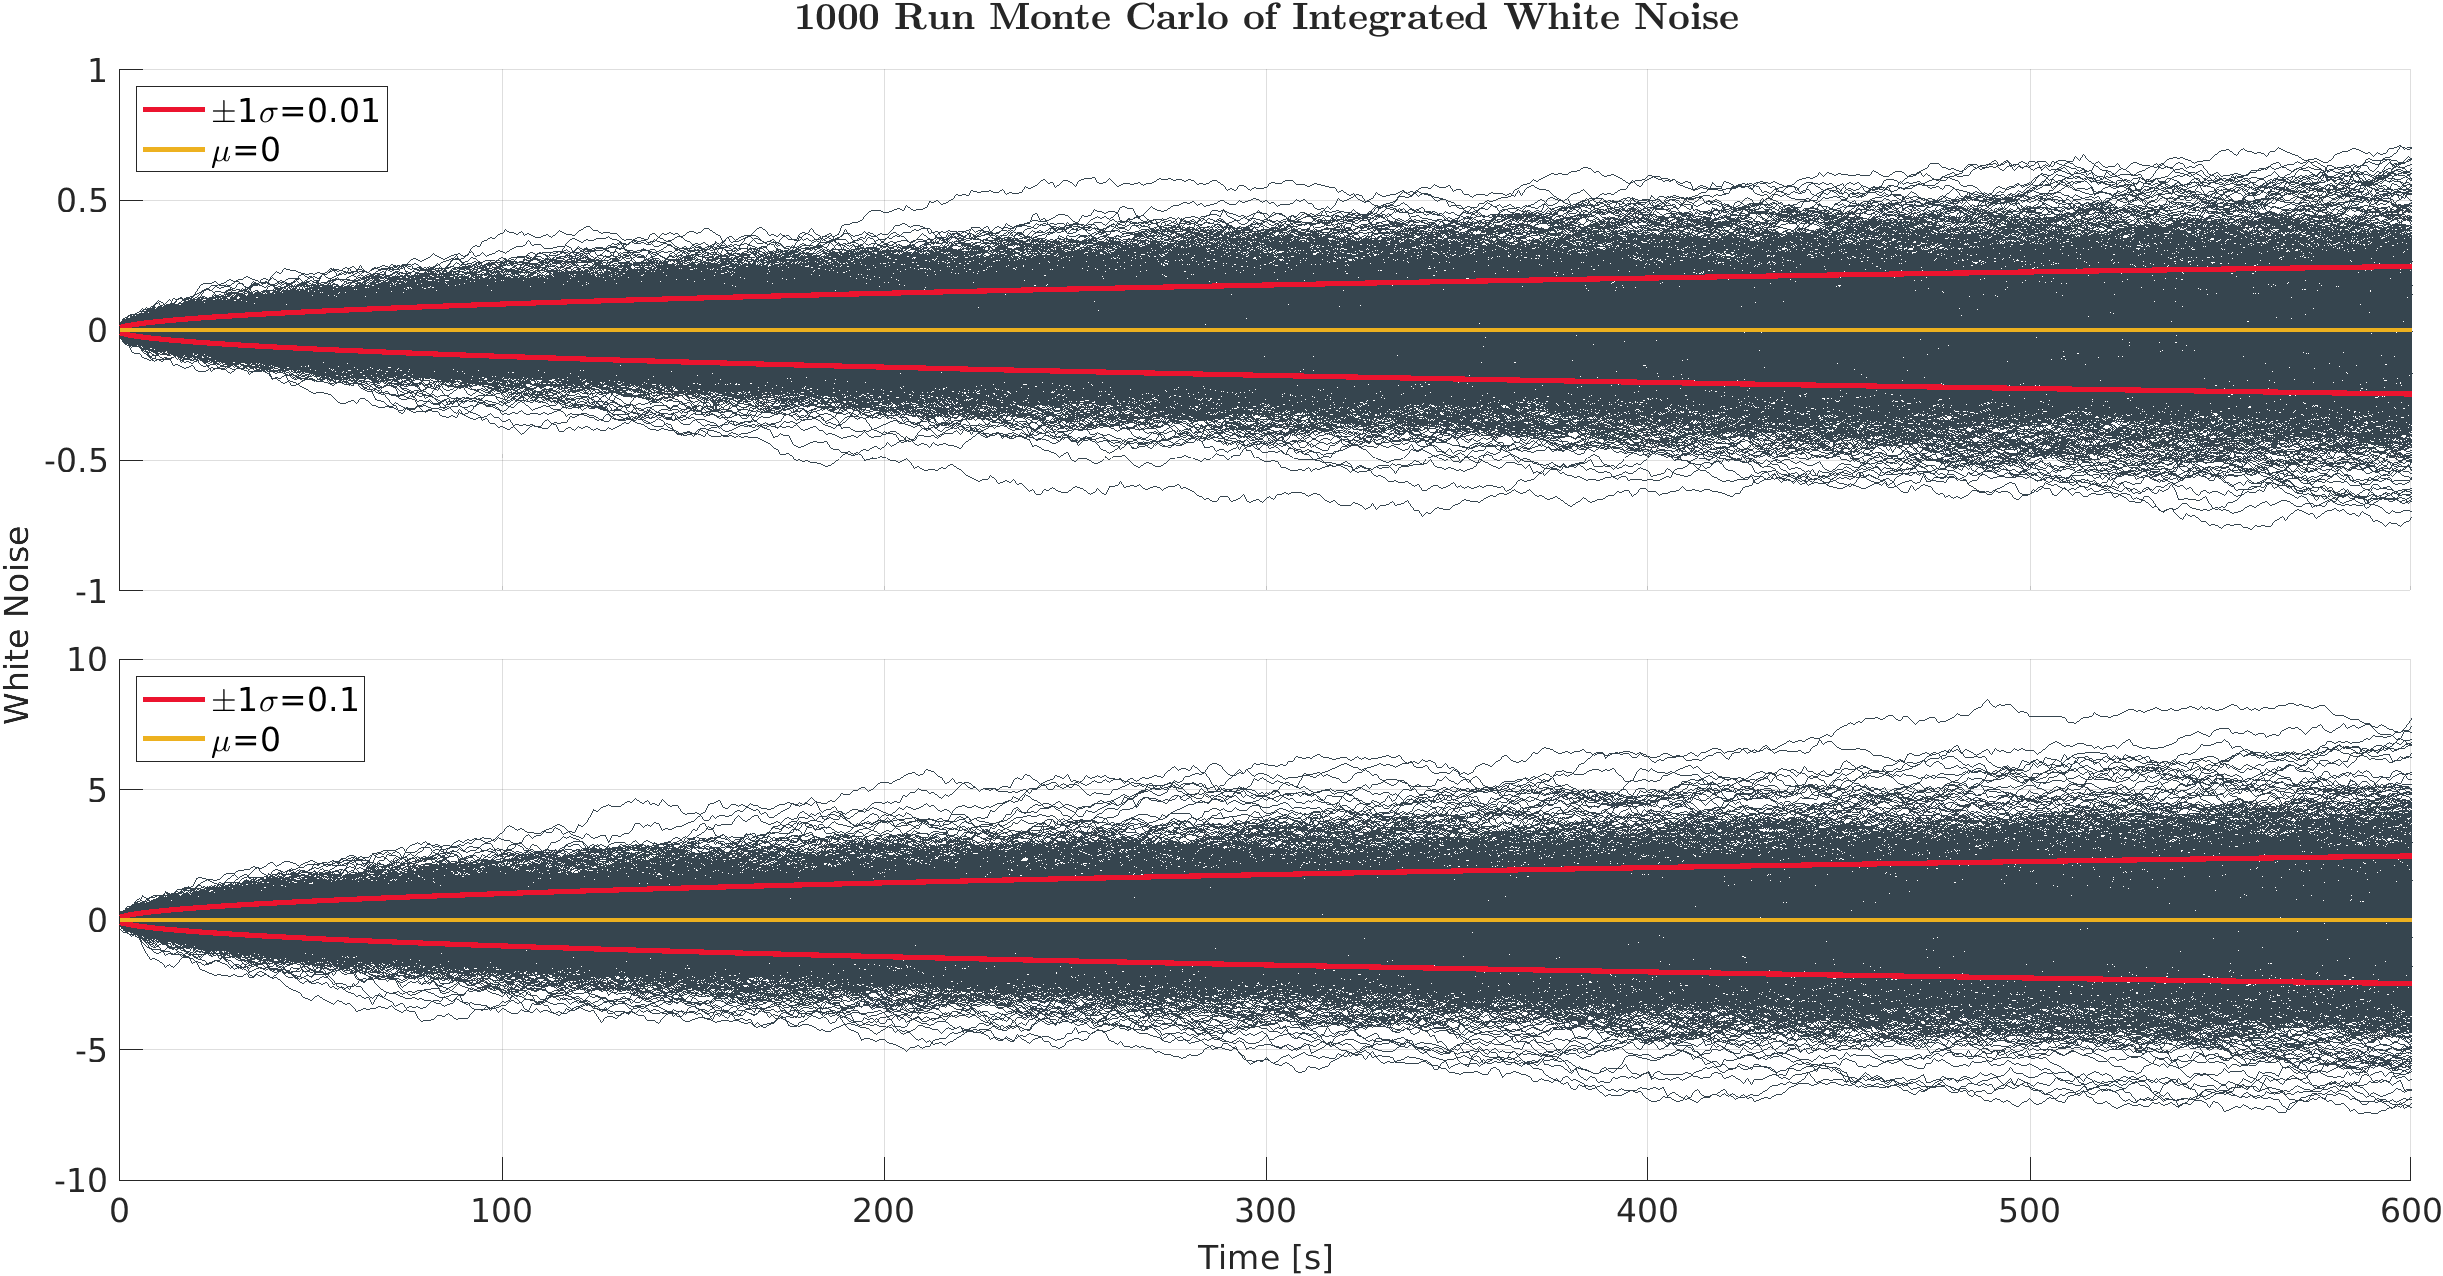
\includegraphics[width=0.85\textwidth]{1b.png}
    \caption{Integrated White Noise.}
  \end{figure}
  \begin{lstlisting}
  time = 0:10*60;
  dt = 1;
  noise = [0.01, 0.1];
  w = zeros(1000, length(time), 2);
  sig = zeros(length(time), 2);
  sig_mc = zeros(length(time), 2);
  mu = zeros(length(time), 2);
  mu_mc = zeros(length(time), 2);
  % 2 standard deviations
  for n = 1:2
      % 1000 MC runs
      for m = 1:1000
          % 10 minute run
          for t = 1:length(time)
              if t == 1
                  w(m,t,n) = noise(n)*randn;
                  sig(t,n) = noise(n) * dt * sqrt(t);
              else
                  w(m,t,n) = w(m,t-1,n) + noise(n)*randn;
                  sig(t,n) = noise(n) * dt * sqrt(t);
              end
          end
      end
  end
  \end{lstlisting}
  Performing a similar monte carlo simulation on a first order markov process 
  with varying time constants.
  \begin{figure}[H]
    \centering
    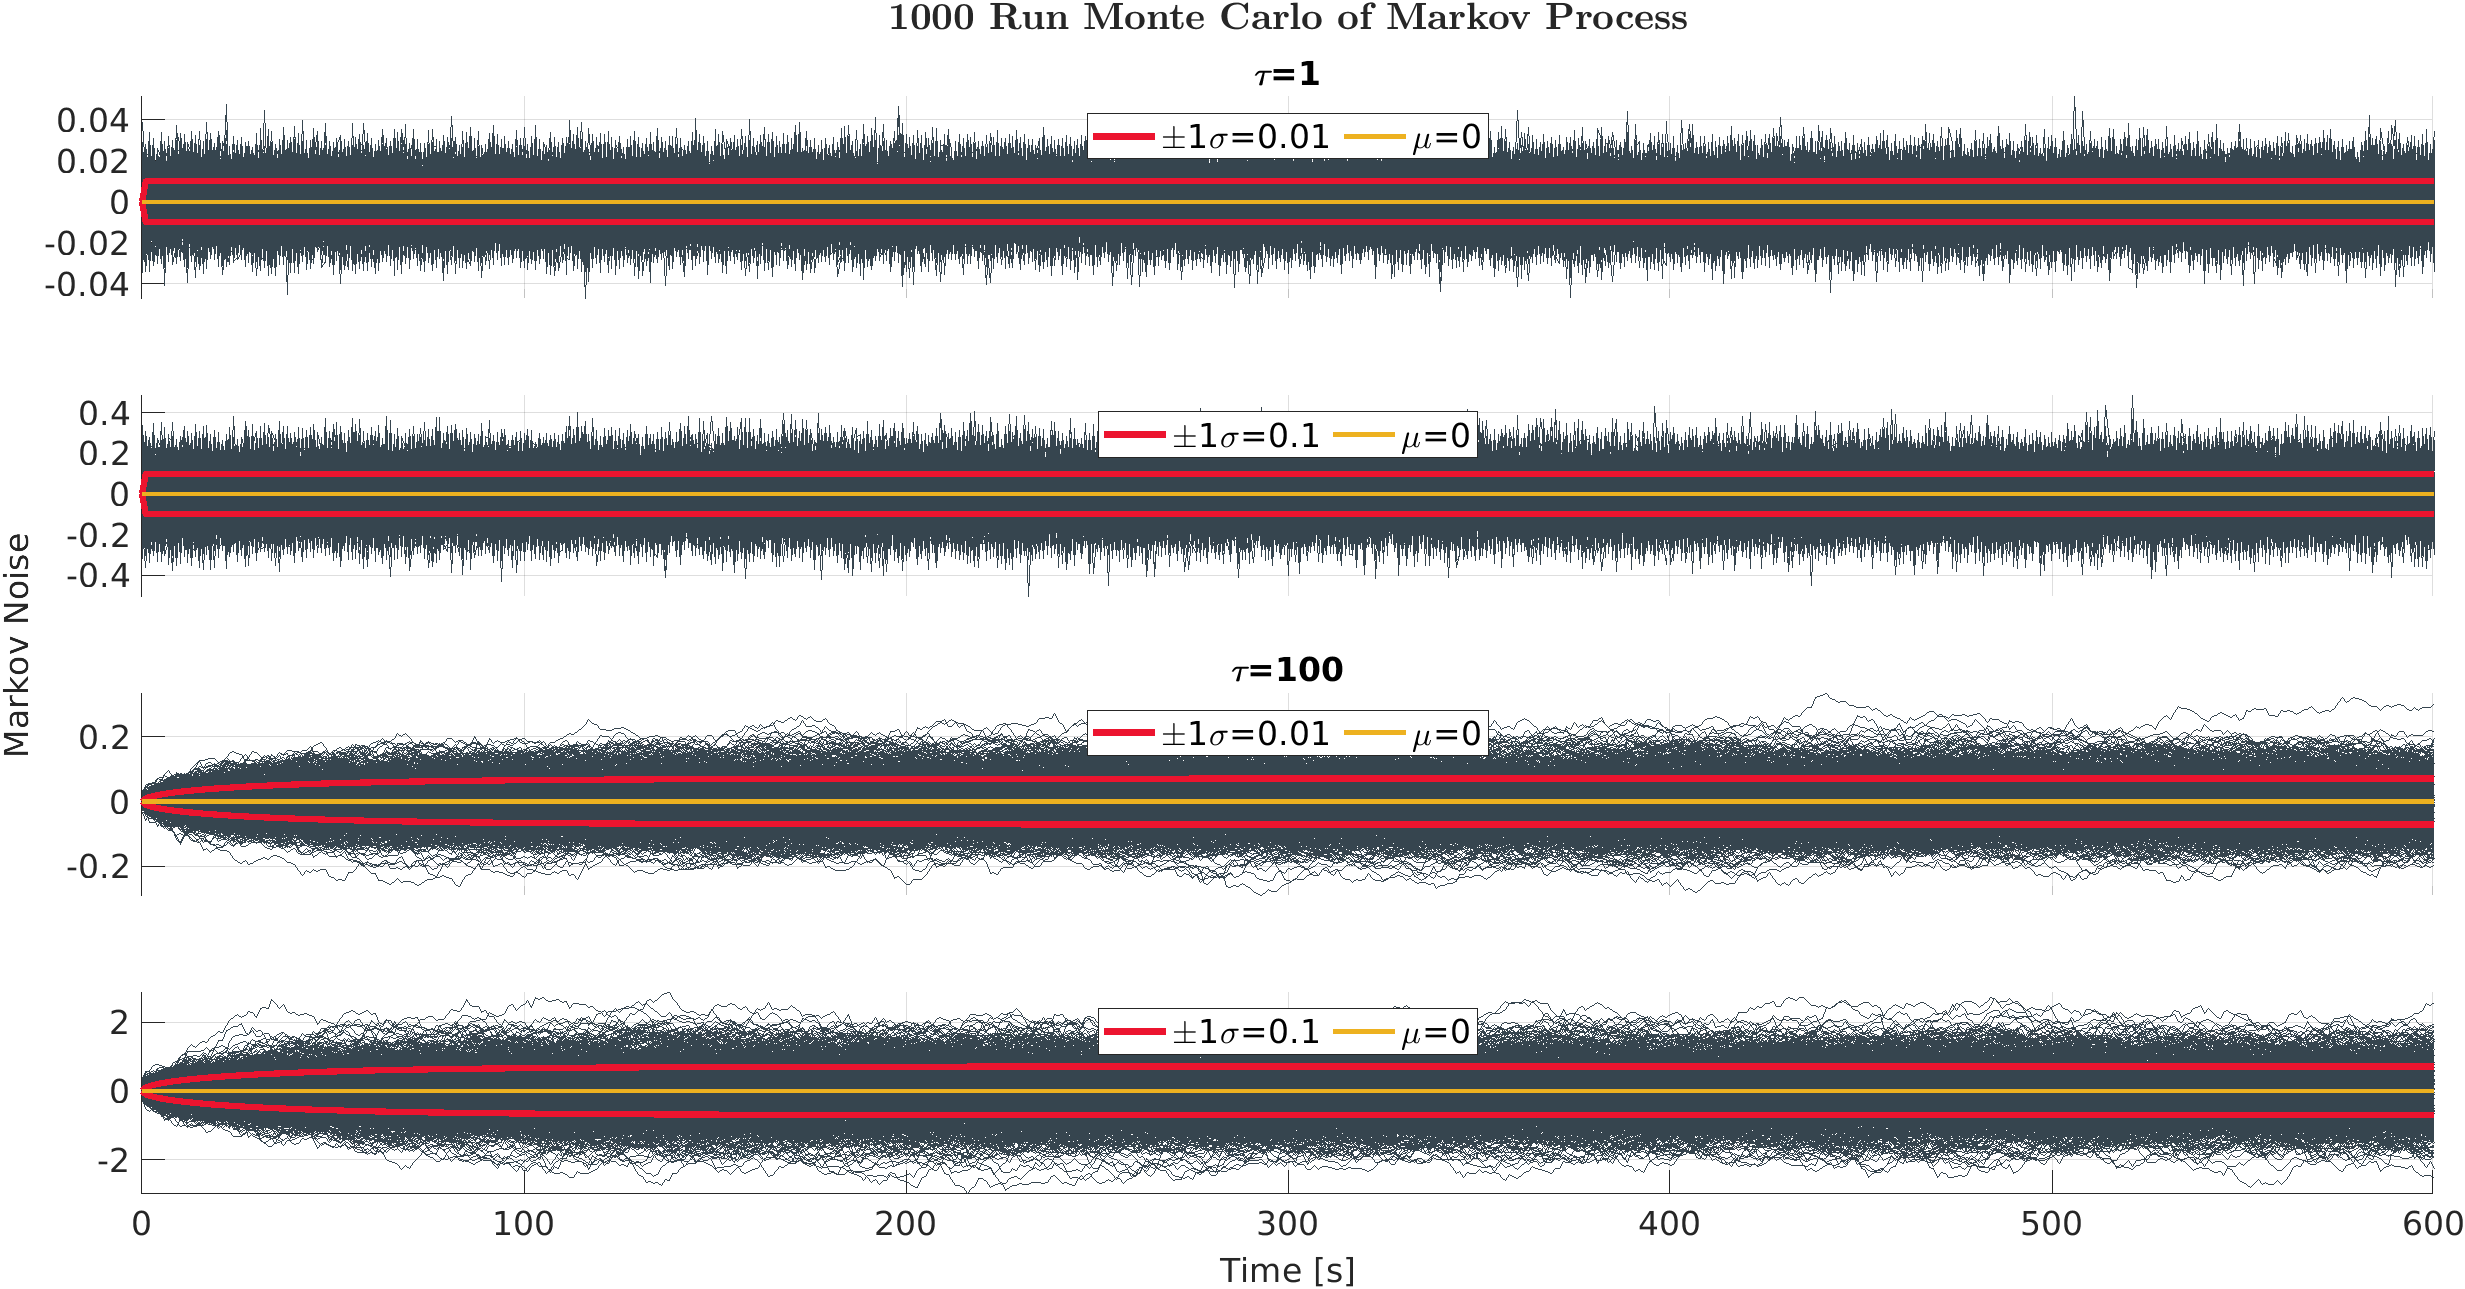
\includegraphics[width=0.85\textwidth]{1c.png}
    \caption{Markov Process Noise.}
  \end{figure}
  \begin{lstlisting}
  time = 0:10*60;
  dt = 1;
  noise = [0.01, 0.1];
  time_const = [1, 100];
  x = zeros(1000, length(time), 4);
  sig = zeros(length(time), 4);
  sig_mc = zeros(length(time), 4);
  mu = zeros(length(time), 4);
  mu_mc = zeros(length(time), 4);
  % 2 standard deviations
  for i = 1:2
      n = noise(i);
      % 2 time constants
      for s = 1:2
          tau = time_const(s);
          if i == 1
              ii = i + s - 1;
          else
              ii = i + s;
          end
          % 1000 MC runs
          for m = 1:1000
              % 10 minute run
              for t = 1:length(time)
                  w = n*randn;
                  if t == 1
                      x(m,t,ii) = w*dt;
                  else
                      xDot = -x(m,t-1,ii)/tau + w;
                      x(m,t,ii) = x(m,t-1,ii) + xDot*dt;
                  end
                  A = 1 - (dt / tau);
                  sig(t,ii) = n * dt * sqrt((A^(2*time(t)) - 1) / (A^2 - 1));
              end
          end
      end
  end
  \end{lstlisting}
  As shown, while the larger time constant makes the standard deviation 
  grow more gradually, the magnitude of the errors are significantly larger. 
  The noise with the time constant of 1 almost instantly grows to its 
  maximum threshold. Errors due to larger standard deviation values also 
  prove to result in larger values. The markov process is also zero mean.

  % PROBLEM 2
  \vspace{24pt}
  \item Determine the expected uncertainty for an L1-L5 ionosphere free 
  pseudorange measurement and L2-L5 ionosphere free pseudorange. Assuming 
  all measurements have the same accuracy (L1, L2, L5) which will provide 
  the best ionosphere estimate?
  \\ \solution
  In order to create an ionosphere free psuedorange, the following formula 
  can be used with respect the the different GPS carrier frequencies and 
  psuedorange measurements.
  \begin{equation*}
    \rho_{IF} = \dfrac{f_a^2}{f_a^2-f_b^2}\rho_a - \dfrac{f_b^2}{f_a^2-f_b^2}\rho_b
  \end{equation*}
  Solving for the L1-L5 measurement:
  \begin{equation*}
    \begin{split}
      \rho_{IF} &= \dfrac{(1575.42(10^6))^2}{(1575.42(10^6))^2-(1176.45(10^6))^2}\rho_{L1} - \dfrac{(1176.45(10^6))^2}{(1575.42(10^6))^2-(1176.45(10^6))^2}\rho_{L5} \\
      &= 2.2606\rho_{L1} - 1.2606\rho_{L5} \\
      \scriptstyle E\{(\rho_{IF} - \bar{\rho}_{IF})^2\} &= 
      \scriptstyle 5.11\rho_{L1}^2 - 5.69\rho_{L1}\rho_{L5} - 10.22\rho_{L1}\bar{\rho}_{L1} + 5.69\rho_{L1}\bar{\rho}_{L5} + 1.58\rho_{L5}^2 + 5.69\rho_{L5}\bar{\rho}_{L1} - 3.17\rho_{L5}\bar{\rho}_{L5} + 5.11\bar{\rho}_{L1}^2 - 5.69\bar{\rho}_{L1}\bar{\rho}_{L5} + 1.58\bar{\rho}_{L5}^2 \\
      &= E\{5.1103(\rho_{L1}^2-\bar{\rho}_{L1}^2) + 1.5891(\rho_{L5}^2-\bar{\rho}_{L5}^2)\} \\
      &= 5.1103\sigma_{L1}^2 + 1.5891\sigma_{L5}^2 \\
      &= \sigma_{IF,L1L5}^2
    \end{split}
  \end{equation*}
  Similarly:
  \begin{equation*}
    \begin{split}
      \sigma_{IF,L2L5}^2 &= 150.1928\sigma_{L2}^2 + 126.6822\sigma_{L5}^2\\
      \sigma_{IF,L1L2}^2 &= 6.4807\sigma_{L1}^2 + 2.3893\sigma_{L2}^2
    \end{split}
  \end{equation*}
  Assuming a 1-sigma value of 1, the standard deviations are as follows:
  \begin{equation*}
    \begin{split}
      \sigma_{IF,L1L5} &= 2.5883 \:\si{m}\\
      \sigma_{IF,L2L5} &= 17.3316 \:\si{m}\\
      \sigma_{IF,L1L2} &= 2.9782 \:\si{m}
    \end{split}
  \end{equation*}
  This concludes that the L1-L5 combination would provide the best measurement.

  % PROBLEM 3
  \vspace{24pt}
  \item Show that the differential GPS problem is linear. In other words 
  derive the following expression:
  \begin{equation*}
    \delta \rho = 
    \begin{bmatrix}
      uv_x & uv_y & uv_z & 1
    \end{bmatrix}
    \begin{bmatrix}
      r_x \\ r_y \\\ r_z \\ c \delta t_{ab}
    \end{bmatrix}
  \end{equation*}
  \solution
  To solve for the delta psuedorange, each individual psuedorange is considered.
  \begin{equation*}
    \begin{split}
      \rho_a^j &= R_a^j + c(t_a-t^j) + I^j + T^j + \nu_a^j \\
      \rho_b^j &= R_b^j + c(t_b-t^j) + I^j + T^j + \nu_b^j \\
    \end{split}
  \end{equation*}
  Assuming each psuedorange has the same noise characteristics as well as 
  equivalent atmospheric errors, when differencing the psuedoranges:
  \begin{equation*}
    \begin{split}
      \rho_a^j - \rho_b^j = R_a^j - R_b^j + c(t_a-t_b) + \sqrt{2}\nu^j
    \end{split}
  \end{equation*}
  Taking the partial derivatives of this equation where $u$ is the unit vector 
  between the receiver and satellite, $R$ is the range between the receiver and 
  satellite, and $r$ is the position of the receiver:
  \begin{equation*}
    \begin{split}
      \Delta\rho_{ab}^j = \dfrac{u_a^j}{R_a^j}r_a^j - \dfrac{u_b^j}{R_b^j}r_b^j  + c\Delta t_{ab} + \sqrt{2}\nu^j
    \end{split}
  \end{equation*}
  From here, the small angle approximation can be used because the satellites 
  are extremely far away compared to the distance between the receivers. This 
  simplifies the equation by letting the direction and ranges from each receiver 
  to the satellite be the same. Finishing the solution:
  \begin{equation*}
    \begin{split}
      \Delta\rho_{ab}^j &= \dfrac{u_a^j}{R^j}r_a^j - \dfrac{u_b^j}{R^j}r_b^j  + c\Delta t_{ab} + \sqrt{2}\nu^j \\
      &= \dfrac{u^j}{R^j}\Delta r_{ab} + c\Delta t_{ab} + \sqrt{2}\nu^j \\
      &= uv_x^j\Delta r_x + uv_y^j\Delta r_y + uv_z^j\Delta r_z + c\Delta t_{ab} + \sqrt{2}\nu^j
    \end{split}
  \end{equation*}
  Where $uv$ is the unit vector of each axis between receiver $a$ to a satellite. 
  When generalized to all satellites, it is equivalent the the equation defined 
  in the problem statement. Assuming position $a$ is known, position $b$ can 
  be found by adding $\Delta r_{ab}$ to the known position.

  % PROBLEM 4
  \vspace{24pt}
  \item Set up your own 2D planar trilateration problem. Place the SVs at 
  (0,300) (100,400), (700,400), and (800,300). Generate a range measurement 
  for a base station at (400,0) and a user at (401,0).
  \begin{enumerate}[(a)]
    \itemsep -2pt
    \item Solve for the position of the user using 2 SVs and then 4 SVs 
    assuming no clock errors. How does the PDOP change for the two cases?
    \item Solve for the position of the user assuming you need to solve for 
    the user clock bias. What is the PDOP with all 4 satellites.
    \item Calculate a differential solution between the base and user using 
    a single difference model and assuming you must solve for a clock bias 
    between the base station and user. What is the PDOP with all 4 satellites?
    \item Calculate a differential solution between the base and user using a 
    double difference model to remove the clock bias between the base station 
    and user. What is the PDOP with all 4 satellites?
    \item Assuming the range error is zero mean with unit variance, what is 
    the order of accuracy in the above 4 solution methods?
  \end{enumerate}
  \solution
  The following code was used to generate ranges and calculate the user position 
  assuming there were no clock errors.
  \begin{lstlisting}
  x_sv = [   0, 300; ...
           100, 400; ...
           700, 400; ...
           800, 300];
  x_r = [400, 0];
  x_u = [401, 0];

  R_r = sqrt(sum((x_sv-x_r).^2, 2));
  R_u = sqrt(sum((x_sv-x_u).^2, 2));

  % PART A and B
  x1 = [0;0]; x2 = [0;0];
  e1 = 1; e2 = 1;
  while (e1 > 1e-6)
    % 2 sv solution
    u1 = x_sv(1:2,:) - x1';
    R1 = sqrt(sum(u1.^2,2));
    uv1 = u1./R1;

    H1 = -uv1;
    y1 = R_u(1:2,:) - R1;

    dx1 = pinv(H1)*y1;
    x1 = x1 + dx1;
    e1 = norm(dx1);
  end
  while (e2 > 1e-6)
    % 4 sv solution
    u2 = x_sv - x2';
    R2 = sqrt(sum(u2.^2,2));
    uv2 = u2./R2;

    H2 = -uv2;
    y2 = R_u - R2;

    dx2 = pinv(H2)*y2;
    x2 = x2 + dx2;
    e2 = norm(dx2);
  end
  DOP1 = inv(H1'*H1);
  DOP2 = inv(H2'*H2);
  \end{lstlisting}
  Looking at the dop values for both 2 and 4 satellites, the PDOP changes 
  significantly when the number of satellites is doubled. This is due to 
  the fact that there is large ambiguity in the y-axis when using only the 
  first two satellites, which is fixed utilizing the rest. Still, both solutions 
  provide answers that are extremely close to $x = \begin{bmatrix} 401 & 0 
  \end{bmatrix}$, being less than $10^{14}$ away from the actual answer. 
  \begin{equation*}
    \begin{split}
      PDOP_1 &= 5.0577 \\
      PDOP_2 &= 1.0000 \\
    \end{split}
  \end{equation*}
  Repeating the least squares solution assuming you also have to determine the 
  clock bias first means that the 2 satellite solution will no longer work as 
  there is three unknowns. The position solution remains almost exact for the 
  4 satellite solution where $PDOP = 5.0498$. \\

  Using a single difference solution between the base station and user (as 
  described in problem 3), the estimated user position is $x = \begin{bmatrix} 
  401 & -0.0014 \end{bmatrix}$ and $PDOP = 5.04975$. In this case, a differential solution 
  seems to be worse than a standard solution because there is no source of 
  error in the range measurements. Using the small angle approximation here 
  makes the estimation slightly worse. The code below is for a single difference 
  solution.
  \begin{lstlisting}
  H3 = [(x_sv-x_r)./R_r, ones(4,1)];
  y3 = R_r - R_u;
  dx3 = pinv(H3)*y3;
  x3 = [x_r,0]' + dx3;
  DOP3 = inv(H3'*H3);
  \end{lstlisting}
  Solving using double difference techniques removes the need to calculate a 
  clock bias, but increases the the number of measurements from satellites needed 
  by one due to the differencing of all measurements to a reference. The 
  estimated user position is $x = \begin{bmatrix} 401 & -0.0014 \end{bmatrix}$ 
  and $PDOP = 4.2051$. The code below is for a double difference solution.
  \begin{lstlisting}
  u = (x_sv-x_r)./R_r;
  dR = R_r - R_u;
  H4 = u(2:4,:) - u(1,:);
  y4 = dR(2:4) - dR(1);
  dx4 = pinv(H4)*y4;
  x4 = x_r' + dx4;
  DOP4 = inv(H4'*H4);
  \end{lstlisting}
  Based on the estimations and PDOP estimations, the following is a list of best 
  to worst solution accuracies for this simulated scenario:
  \begin{enumerate}[1.]
    \itemsep -2pt
    \item Perfect Clock (A)
    \item Double Differenced (D)
    \item Imperfect Clock (B)
    \item Single Differenced (C)
  \end{enumerate}
  Looking at the GDOP (which would be equivalent to a covariance with a unit 
  variance) for part B and C does not change this answer as they still have 
  the highest values.

  % PROBLEM 5
  \vspace{24pt}
  \item (Bonus for Undergrads/Required for Grads). Repeat problem $\#$4 using 
  4 and 8 SV positions from Lab $\#$2 (4,7,8,9,16,21,27,30). Comment on any 
  difference or similarities with the planar problem in $\#$3.\\
  \solution
  Finding a spot where both receivers in the dynamic data sets had 8 satellites 
  was difficult, therefore the first timestep this occurred was used. This 
  resulted in satellites [3, 6, 11, 14, 17, 19, 24, 30] being used. Running 
  through the same steps as problem 3, the position outputs on a geoplot are 
  shown below as well as the PDOP values of each part for both 4 and 8 satellites.
  \begin{enumerate}[(a)]
    \itemsep -2pt
    \item $PDOP_{4sv} = 2.7265$ \\ $PDOP_{8sv} = 1.0837$
    \item $PDOP_{4sv} = 3.5137$ \\ $PDOP_{8sv} = 1.7370$
    \item $PDOP_{4sv} = 3.5137$ \\ $PDOP_{8sv} = 1.7370$
    \item $PDOP_{4sv} = 3.3109$ \\ $PDOP_{8sv} = 1.4743$
  \end{enumerate}
  \begin{figure}[H]
    \centering
    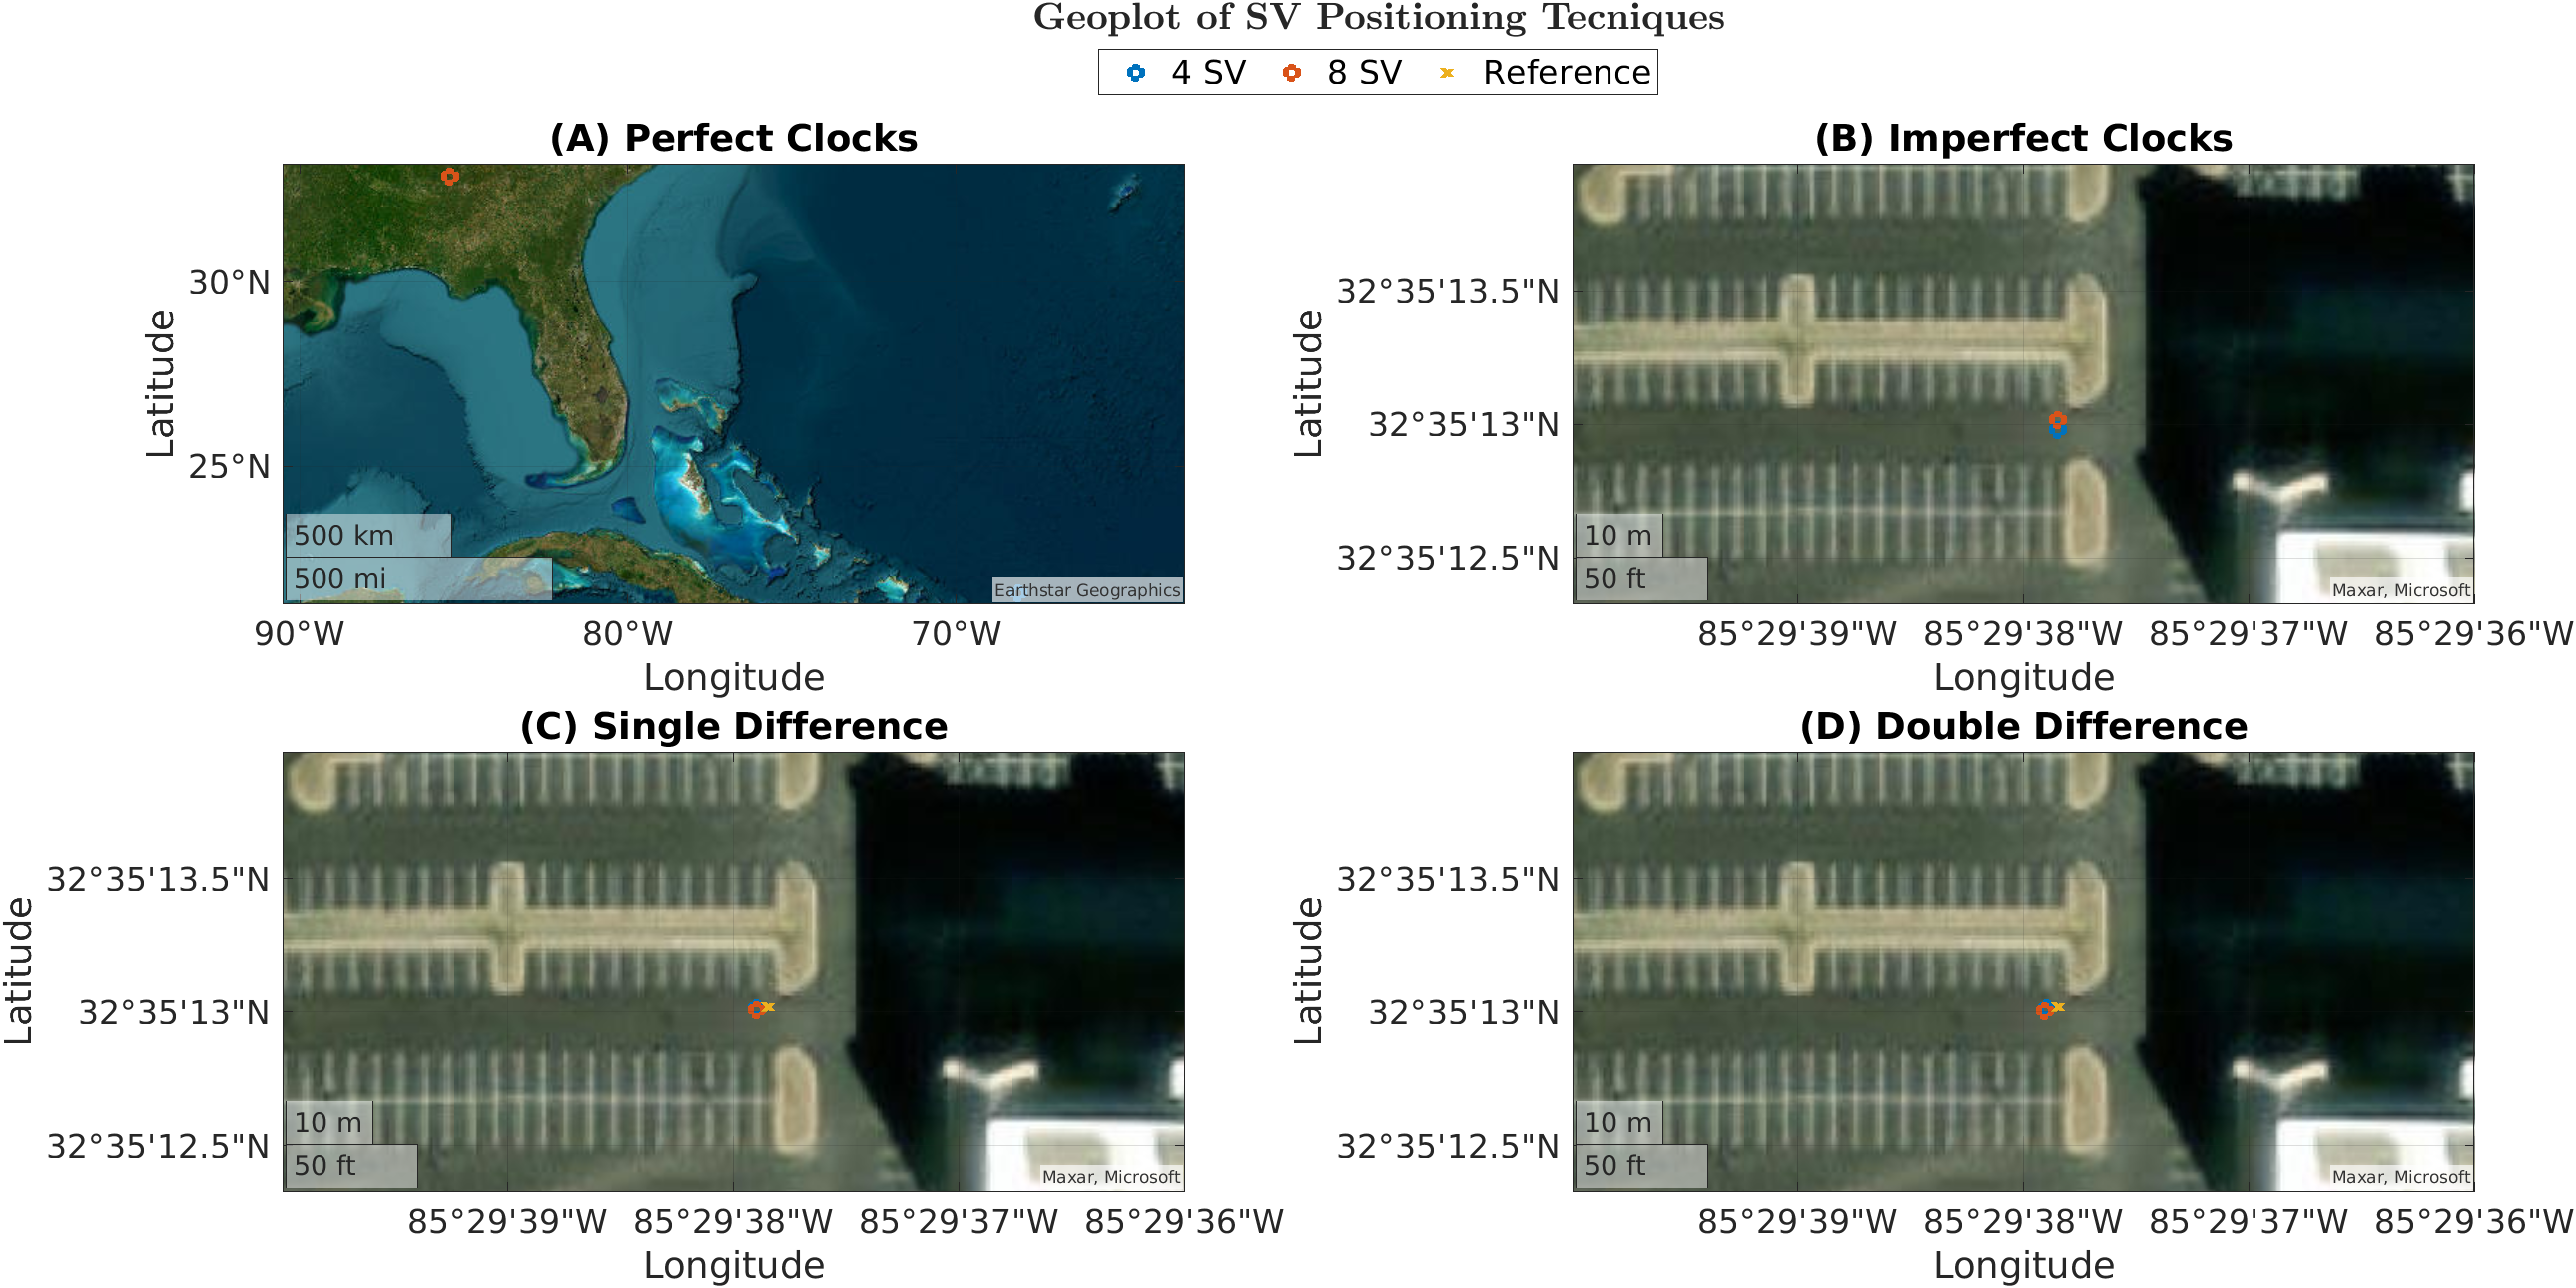
\includegraphics[width=0.85\textwidth]{5.png}
    \caption{Position Estimations with Different Techniques.}
  \end{figure}
  In \emph{part a}, is is obvious that the 4 satellite estimate provides an extremely 
  poor estimate, likely due to a combination of poor satellite geometry and not 
  accounting for clock bias. The 8 satellite geometry provides a more reasonable 
  solution that is tenths or degrees off in latitude and longitude, but provides 
  a height estimate deep inside the earth (-102037m, for reference the 4 SV 
  solution places the receiver at -500793m). Moving to \emph{part b}, accounting 
  for clock bias provides really good positioning. While the PDOP is higher, 
  the position solution is more correct. \emph{Part c} and \emph{part d} also 
  provide good position solutions having the same level of accuracy as \emph{part
  b} (all are in the same area of the MRI building parking lot). The only difference 
  being that the PDOP value for the double differenced solution as smaller. 
  Ranking the solutions by order of accuracy:
  \begin{enumerate}[1.]
    \itemsep -2pt 
    \item Double Differenced (D)
    \item Single Differenced (C)
    \item Imperfect Clock (B)
    \item Perfect Clock (A)
  \end{enumerate}
  While the perfect clock provided the best PDOP values, it is obvious that this 
  values is independent of the actual position solution giving it no bearing on 
  the accuracy.

  % PROBLEM 6
  \vspace{24pt}
  \item Chapter 2, Problem 1a and 1b for PRN\#4. Repeat 1a for PRN \#7. \\
  \solution
  The following is a function made to generate the C/A code for a GPS 
  satellite:
  \begin{lstlisting}
  function G2i = caGen(s1, s2)
  % initialize to all ones
  G1 = ones(1,10);
  G2 = ones(1,10);
  G2i = zeros(1,1023);
  for i = 1:1023
      % create ca code
      G2i(i) = bitSum(G2(s1), G2(s2));
      G2i(i) = bitSum(G2i(i), G1(10));
      % update G1
      newBit = bitSum(G1(3), G1(10));
      G1 = [newBit, G1(1:9)];
      % update G2
      newBit = 0;
      for j = [2,3,6,8,9,10]
          newBit = bitSum(newBit, G2(j));
      end
      G2 = [newBit, G2(1:9)];
  end
  % XOR function
  function s = bitSum(a,b)
      s = a+b;
      if s > 1
          s = 0;
      end
  end
  end
  \end{lstlisting}
  For PRN\#4 the values of $s1$ and $s2$ are 5 and 9, and PRN\#7 they are 
  1 and 8 (provided in the GPS specification document 
  \url{https://www.gps.gov/technical/icwg/IS-GPS-200N.pdf}). Plotting the first 
  and last 16 chips of PRN\#4 and PRN\#7:
  \begin{figure}[H]
    \centering
    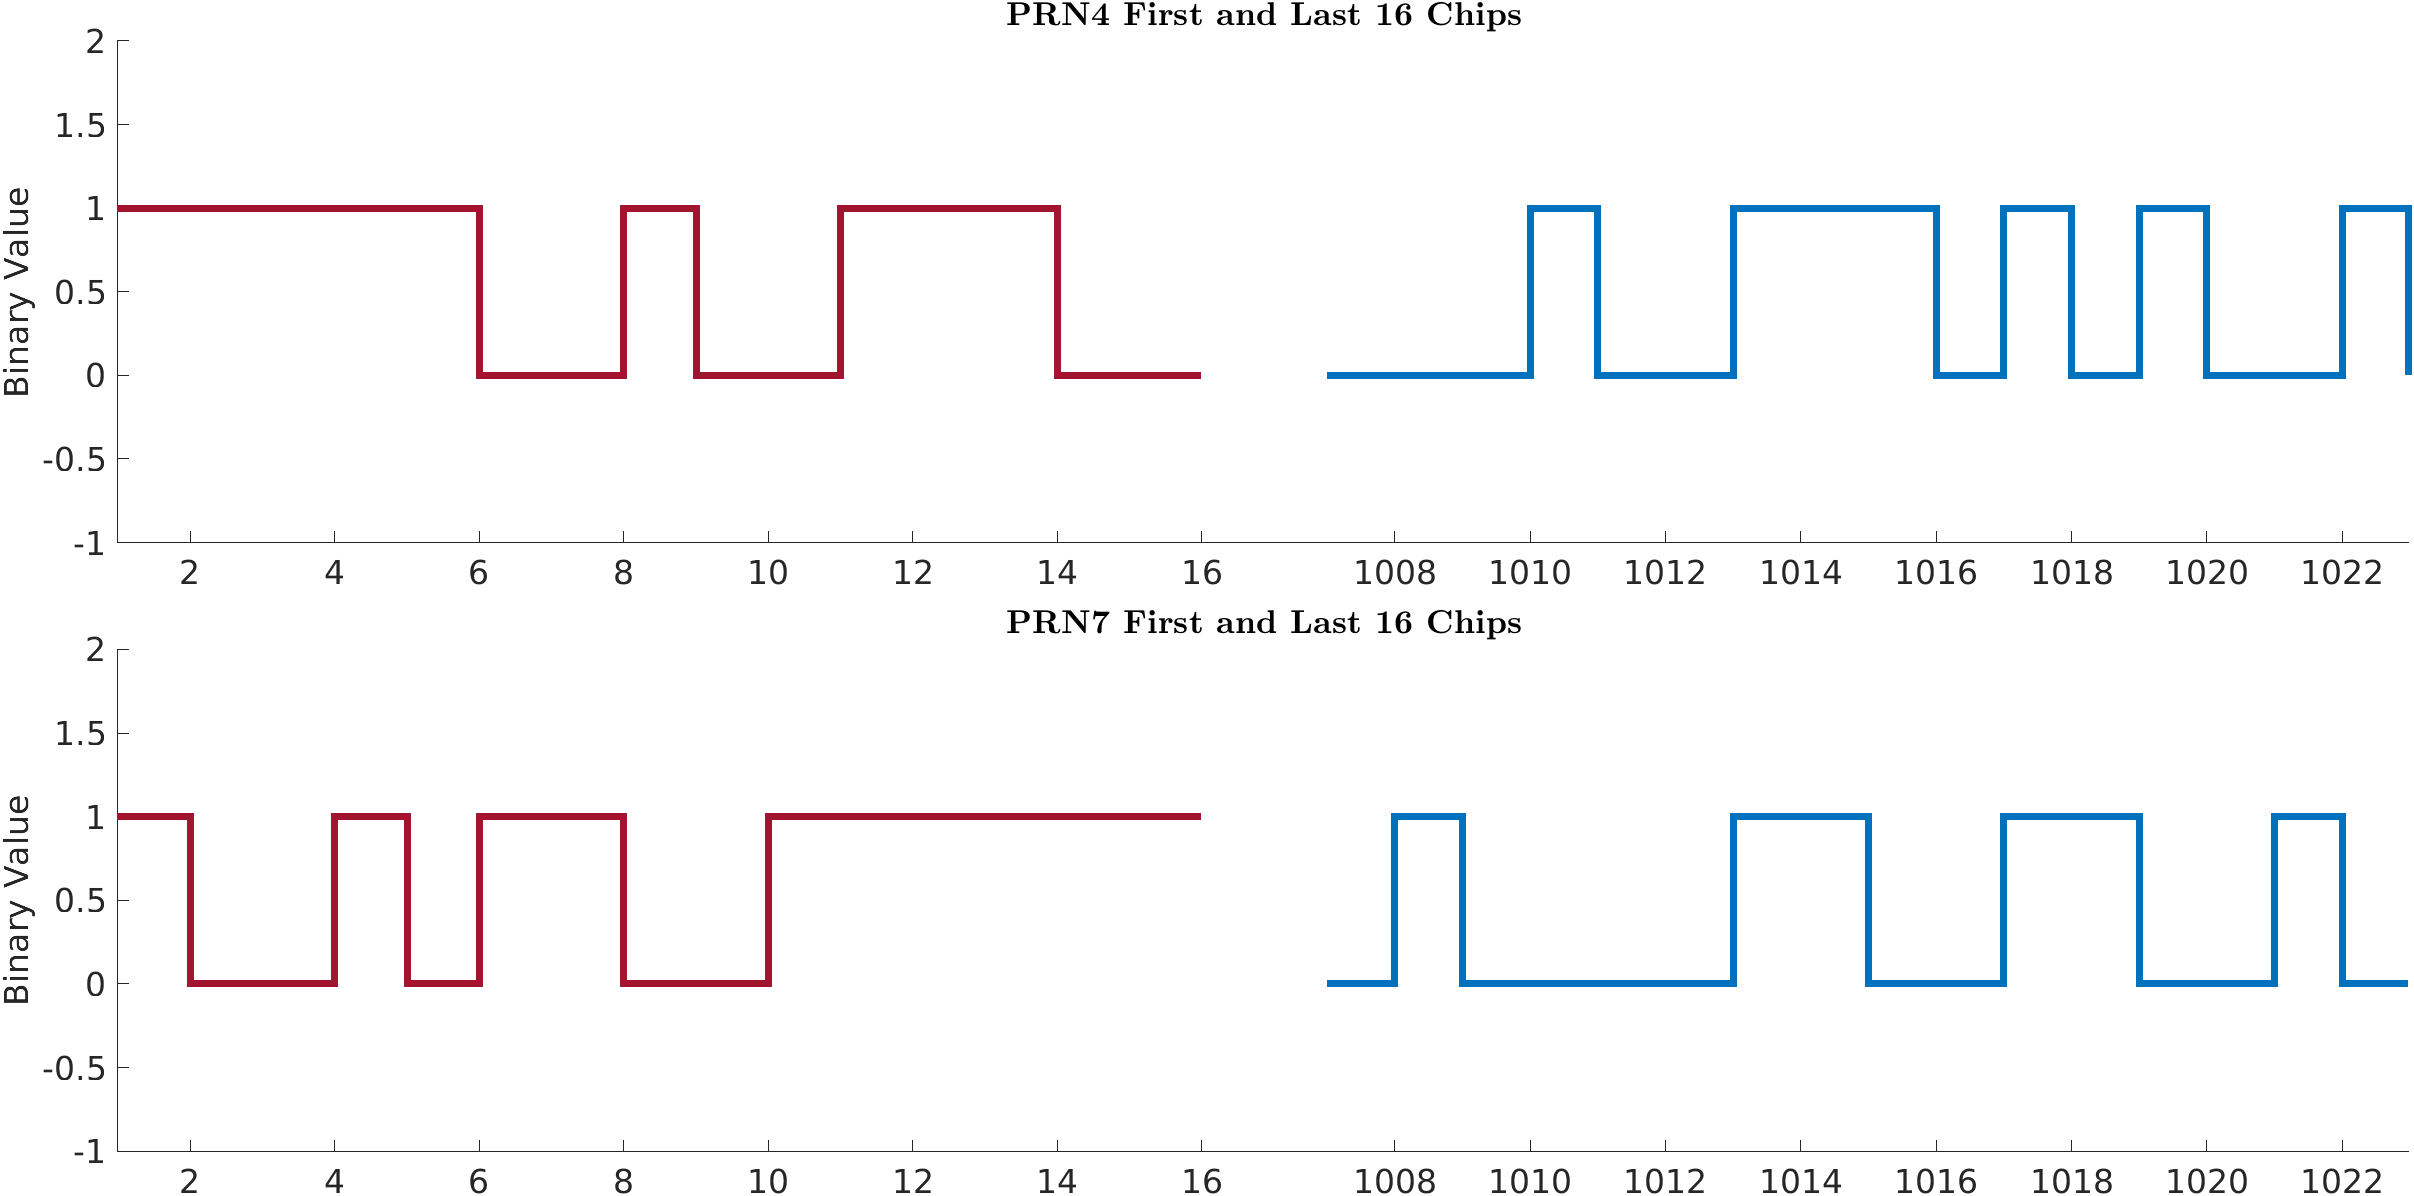
\includegraphics[width=0.85\textwidth]{6a.png}
    \caption{Beginning and Ending Chips of PRNs.}
  \end{figure}
  Since the PRNs repeat every 1023 chips, the C/A code should repeat in chips 
  1023-2046. Verifying this by duplicating the code above and running the 
  generator twice reveals that the first 16 bits are exactly the same in both 
  sequences. Plotting the autocorrelation between chips 1-1023 and chips 
  1024-2046 of PRN\#4 which confirms that the sequence repeats every 1023 chips:
  \begin{figure}[H]
    \centering
    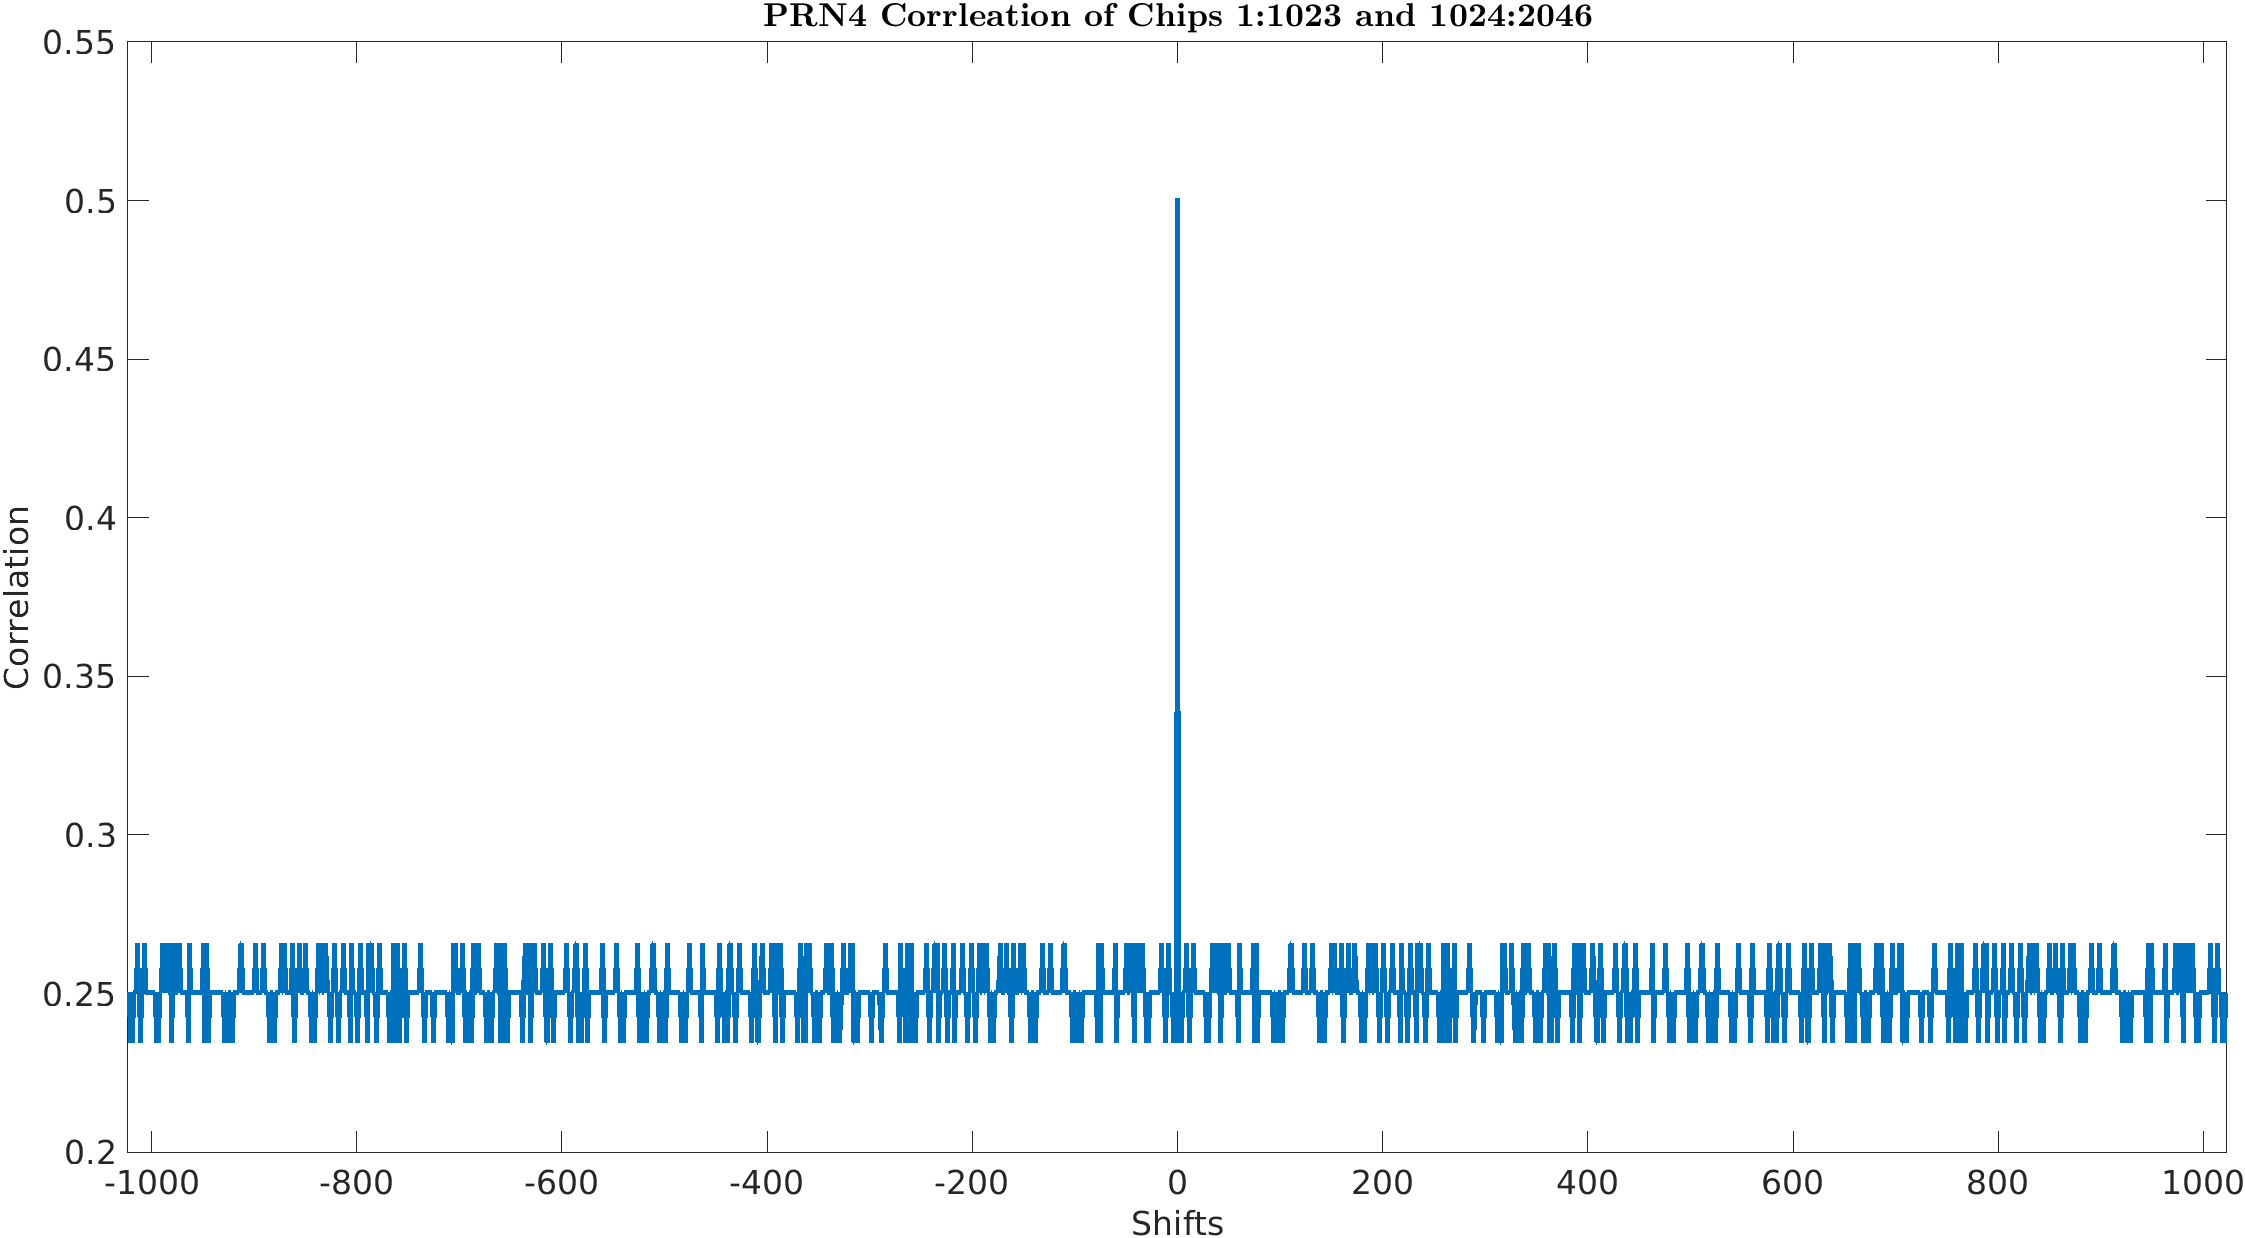
\includegraphics[width=0.85\textwidth]{6b.png}
    \caption{Autocorrelation of PRN\#4 Chips 1-1023 and 1024-2046.}
  \end{figure}
  
  % PROBLEM 7
  \vspace{24pt}
  \item Using your PRN sequence for PRN 4 and 7, repeat problem \#2 from 
  HW\#1. Compare the results to the results for your made up sequence.
  \begin{enumerate}[(a)]
    \item Plot the histogram on each sequence
    \item Plot the spectral analysis on each sequence
    \item Plot the autocorrelation each sequence with itself (i.e. a sequence 
    delay crosscorrelation)
    \item Plot the cross autocorrelation between the two sequences
  \end{enumerate}
  \solution
  Below are the plots for each part and each PRN.
  \begin{figure}[H]
    \centering
    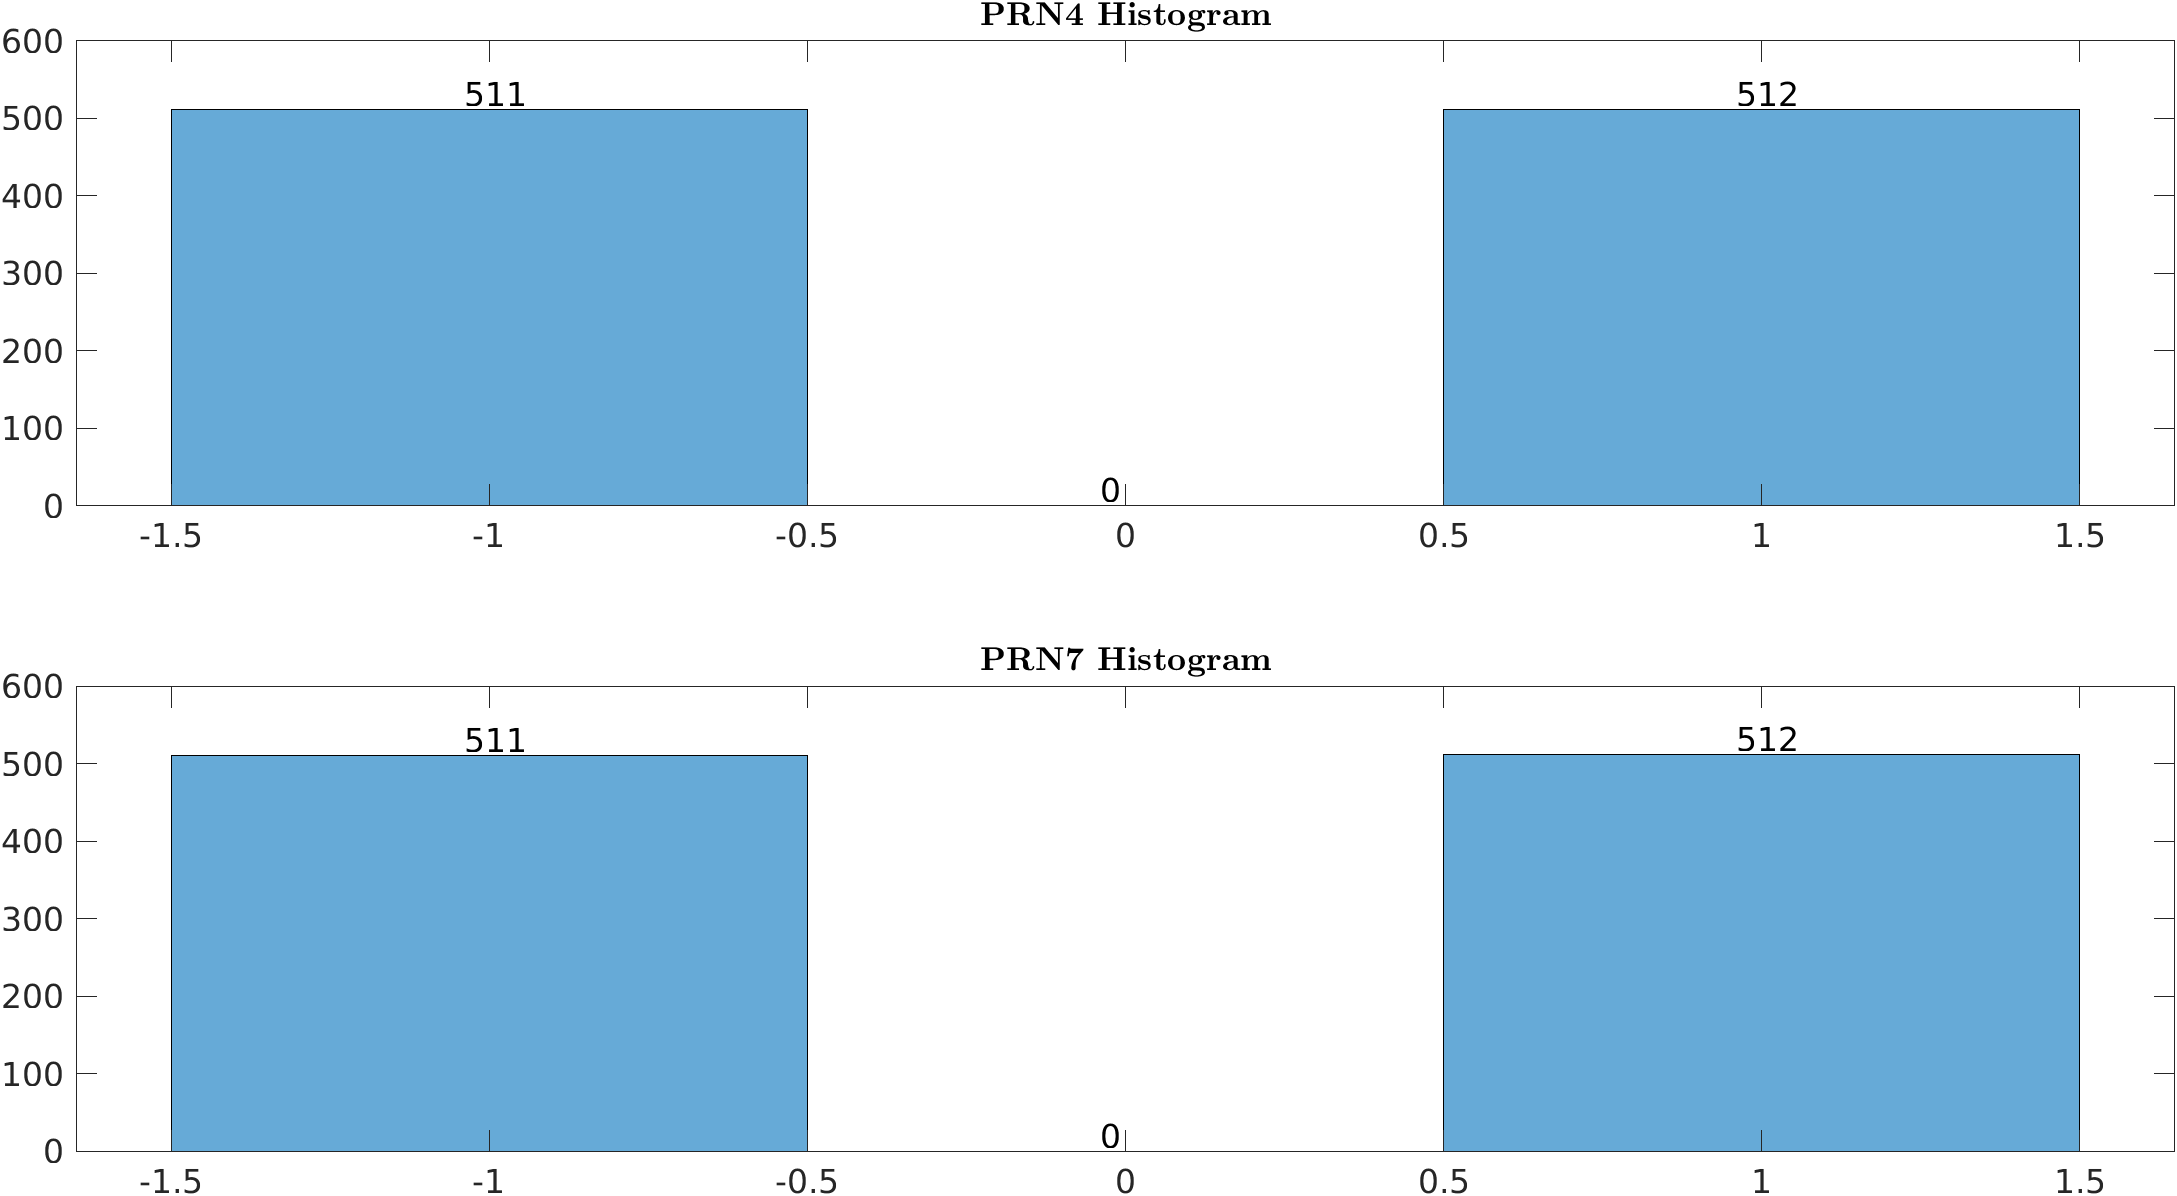
\includegraphics[width=0.85\textwidth]{7a.png}
    \caption{Histograms of PRN\#4 and PRN\#7.}
  \end{figure}
  \begin{figure}[H]
    \centering
    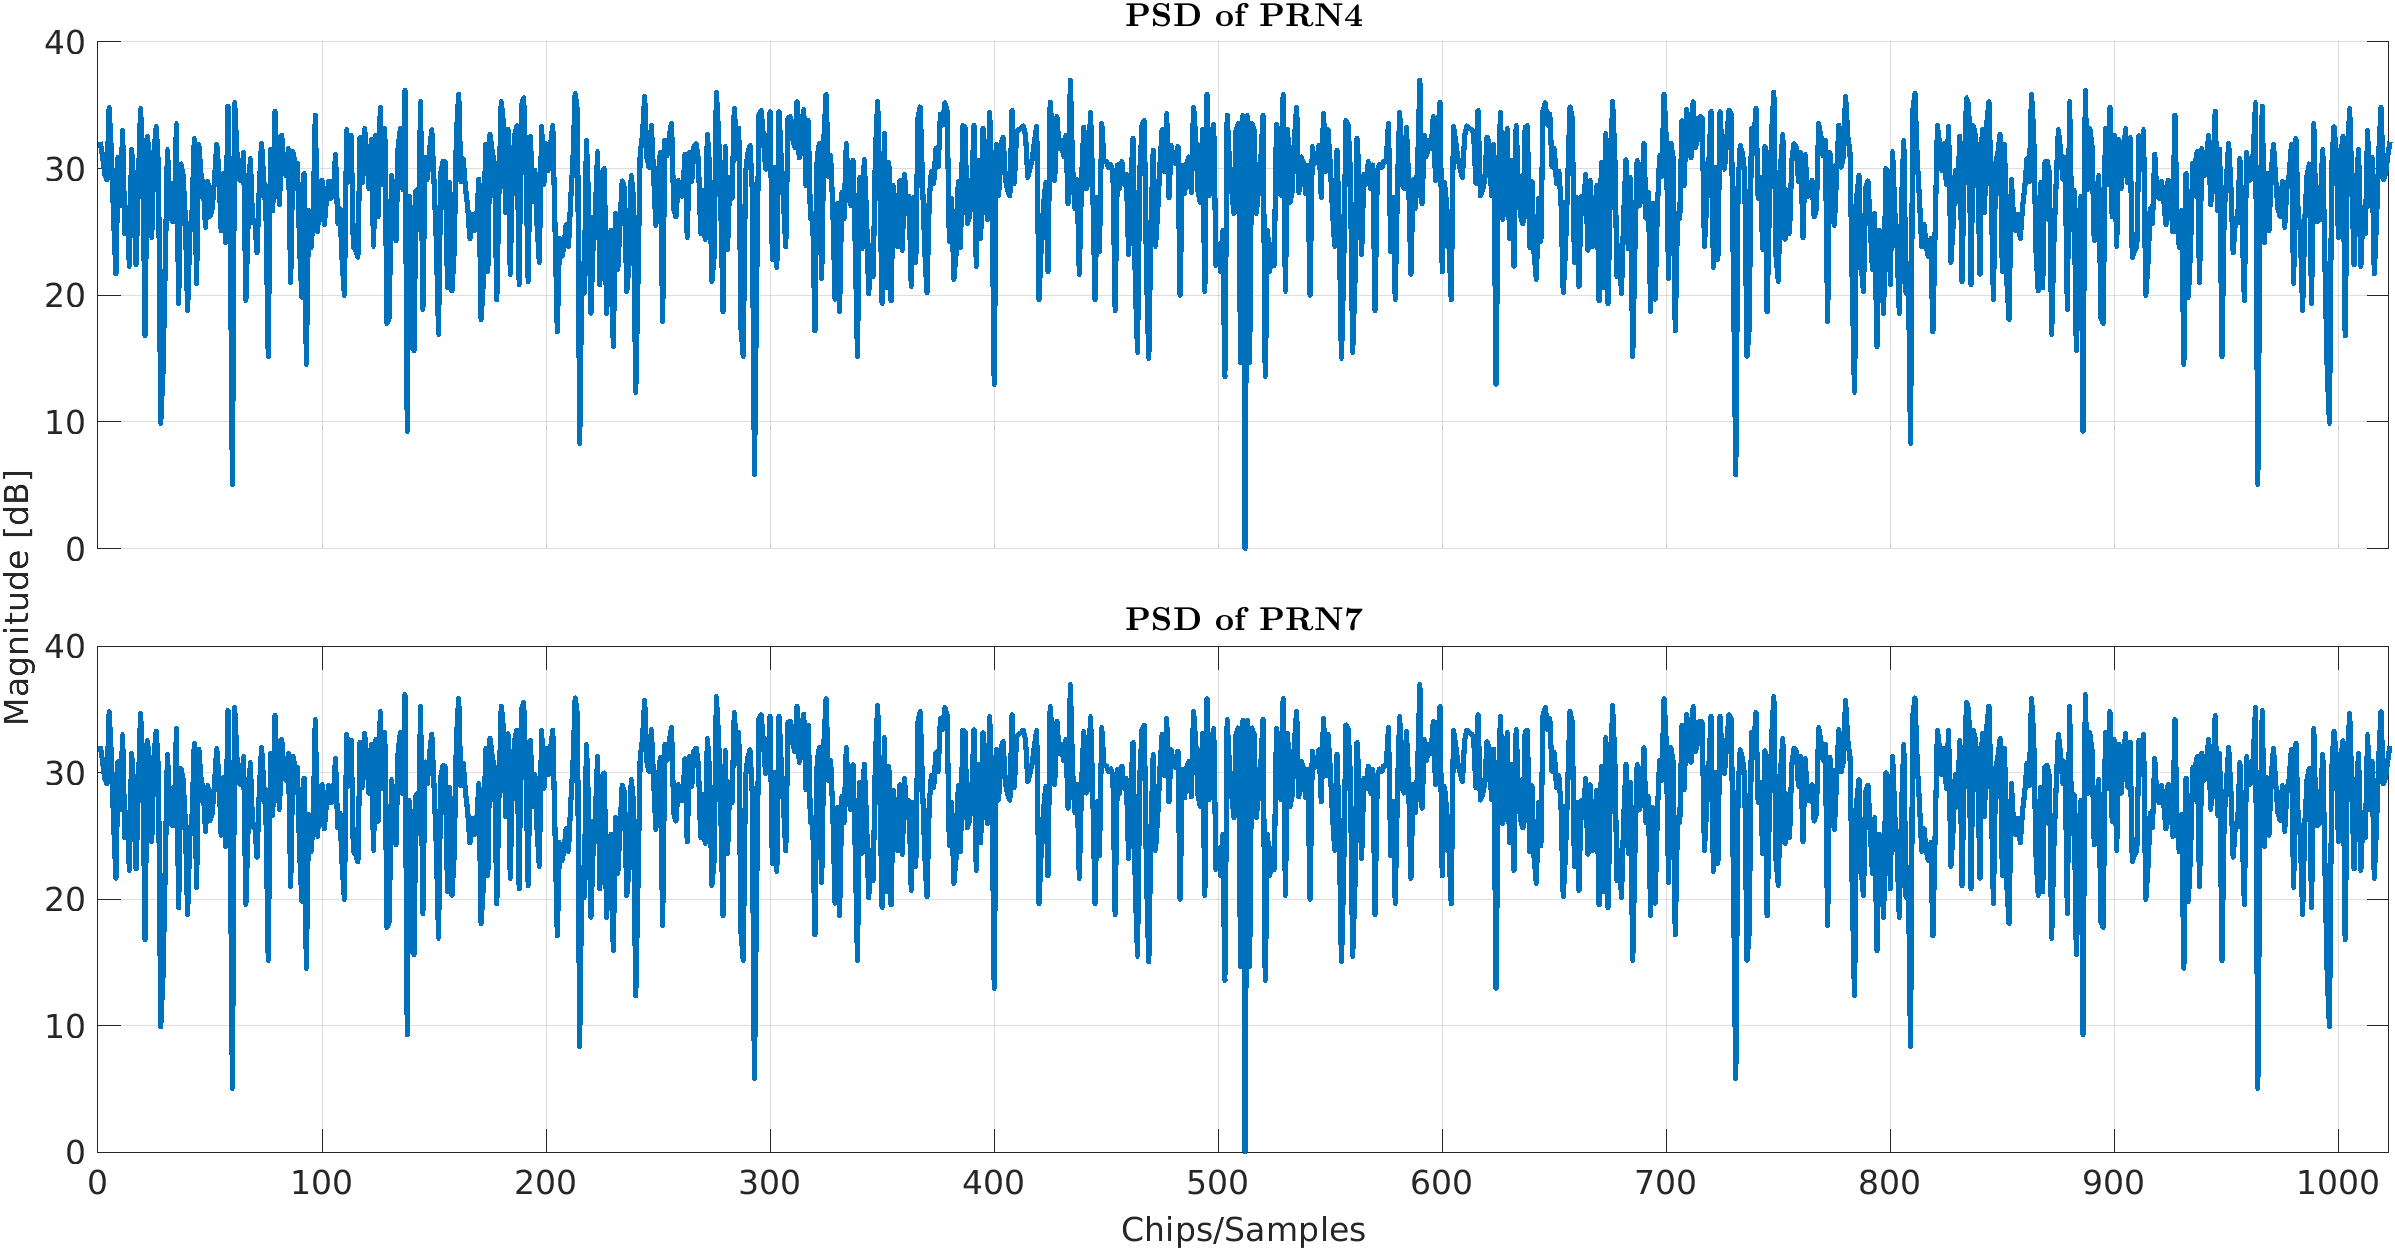
\includegraphics[width=0.85\textwidth]{7b.png}
    \caption{PSDs of PRN\#4 and PRN\#7.}
  \end{figure}
  \begin{figure}[H]
    \centering
    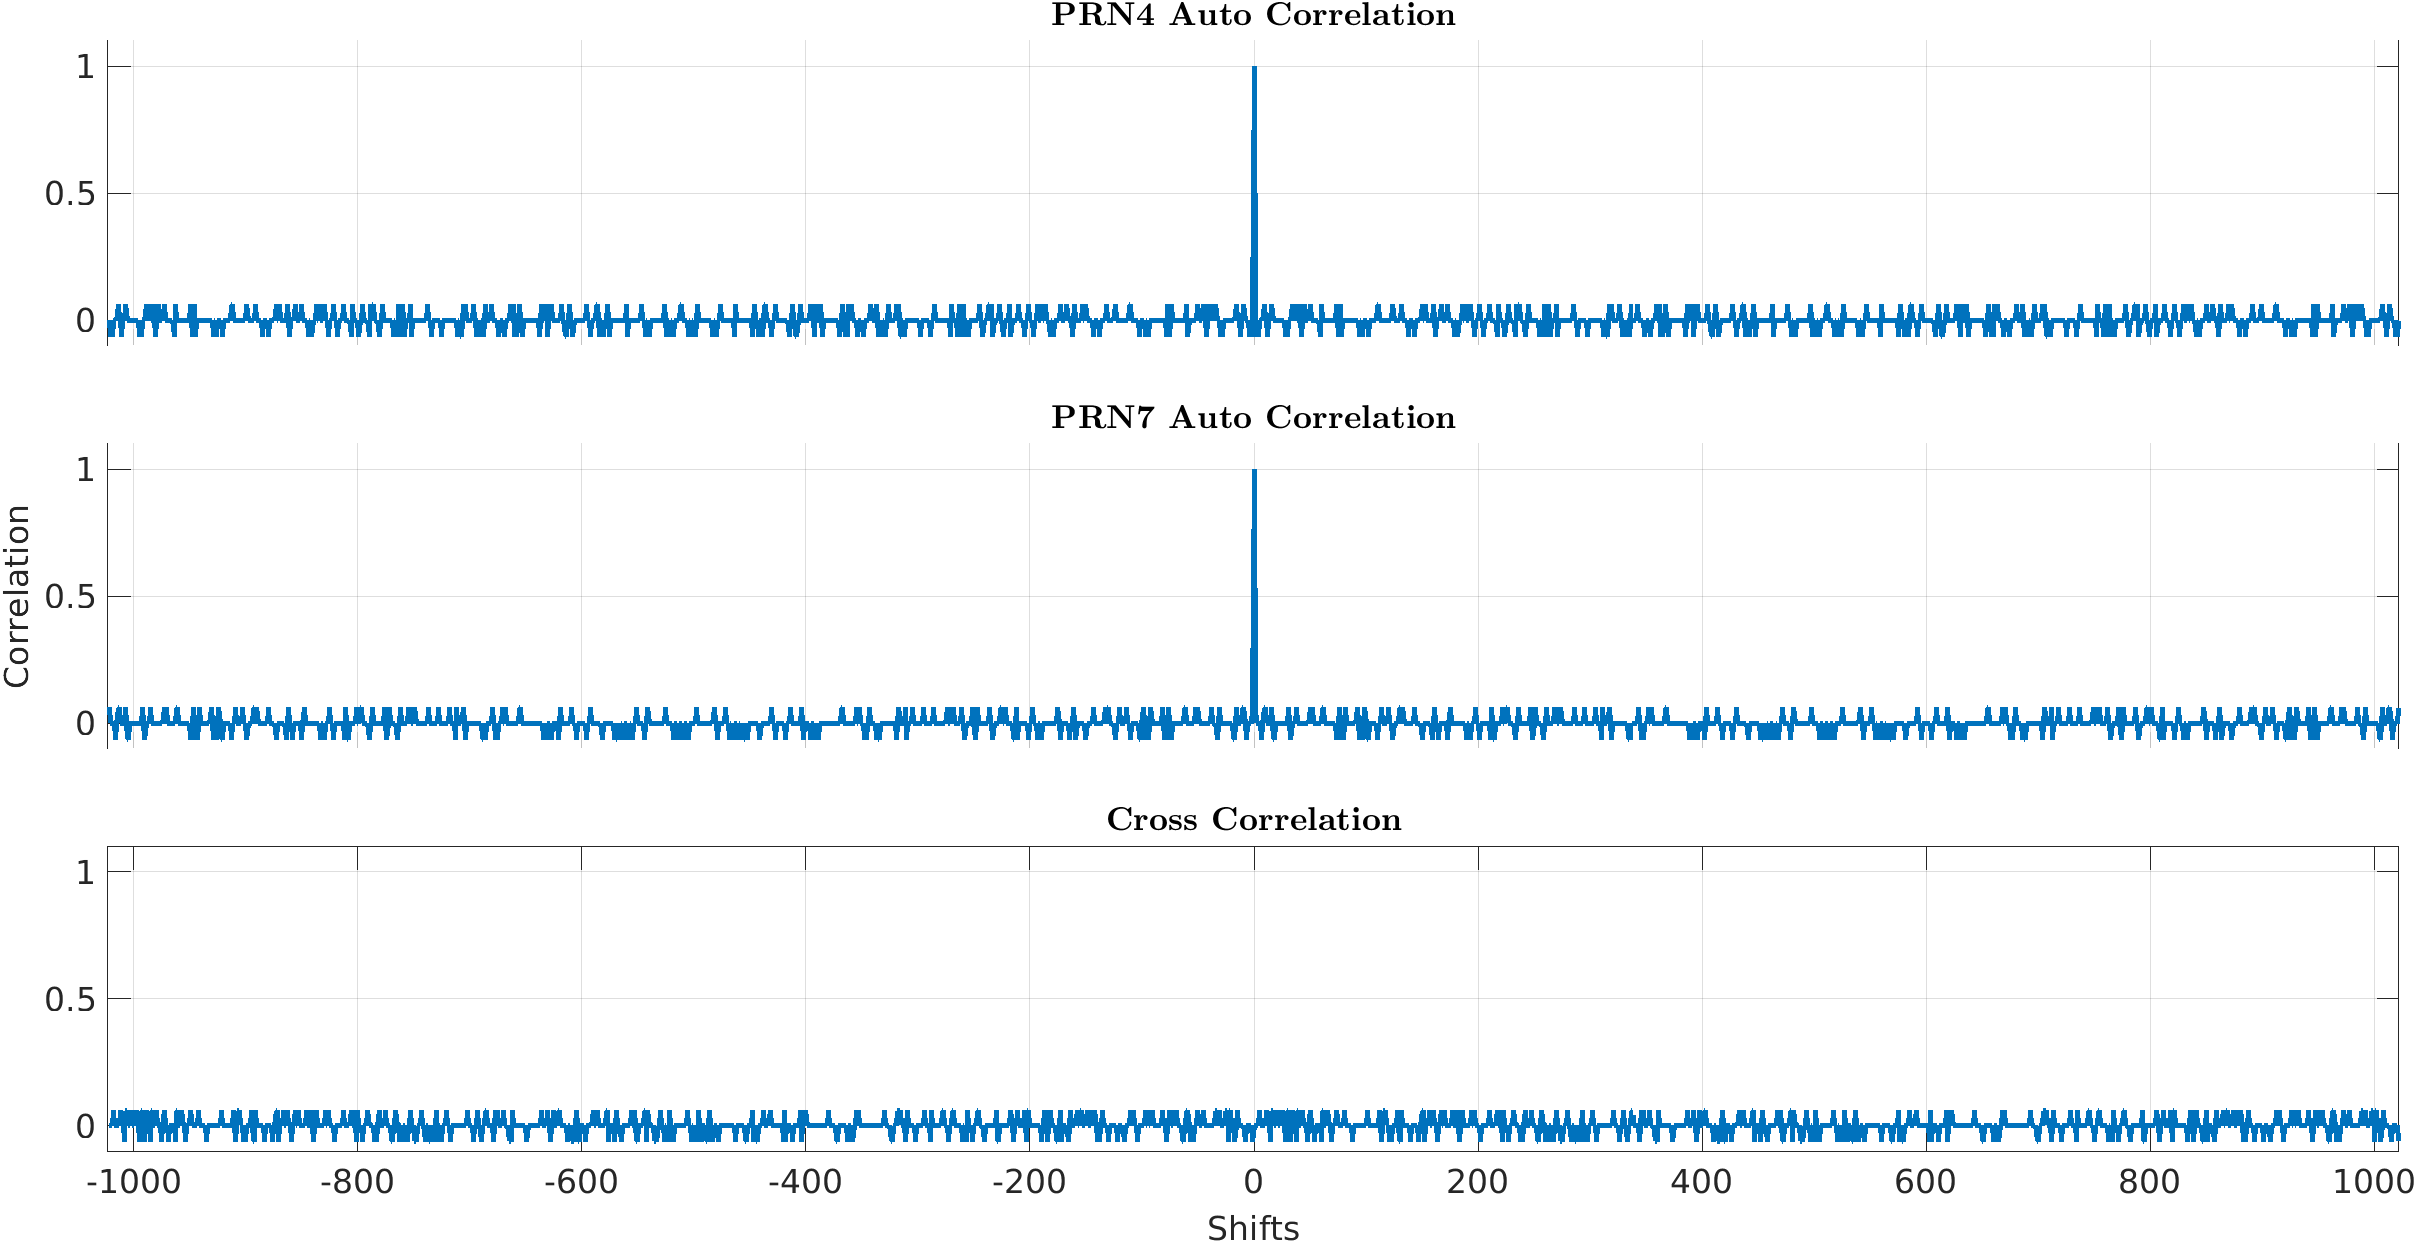
\includegraphics[width=0.85\textwidth]{7c.png}
    \caption{Correlations of PRN\#4 and PRN\#7.}
  \end{figure}
  Looking at the histograms, it is obvious that the assortment of 0 (-1) and 1 
  is super even. The PSD displays that the noise is random on the C/A code with 
  a mean value just under 30. And the correlations prove that each PRN is only correlated with itself at one 
  timepoint and completely uncorrelated with other PRNs. \\

  Comparing these results to those from HW\#1, each of the plots look almost 
  identical (except for the randomness in each one from HW\#1). This proves that 
  GPS PRNs contain the properties of psuedorandom sequences.

  % PROBLEM 8
  \vspace{24pt}
  \item Take your C/A code from problem above (i.e. PRN $\#$4 and $\#$7) and 
  multiply it times the L1 Carrier (your C/A code must be in the form -1 
  and +1). Perform a spectral analysis (magnitude) on the resultant signal. 
  You will need to make sure to “hold” your C/A code bits for the correct 
  length of time (I suggest using a sample rate 10x the L1 carrier frequency 
  - meaning each chip of the C/A code will be used for 10 samples of the sine 
  wave). \\
  \solution
  The following is a PSD of the modulation of the C/A code with the L1 carrier 
  signal. As expected peaks at the L1 carrier frequency for both PRNs.
  \begin{figure}[H]
    \centering
    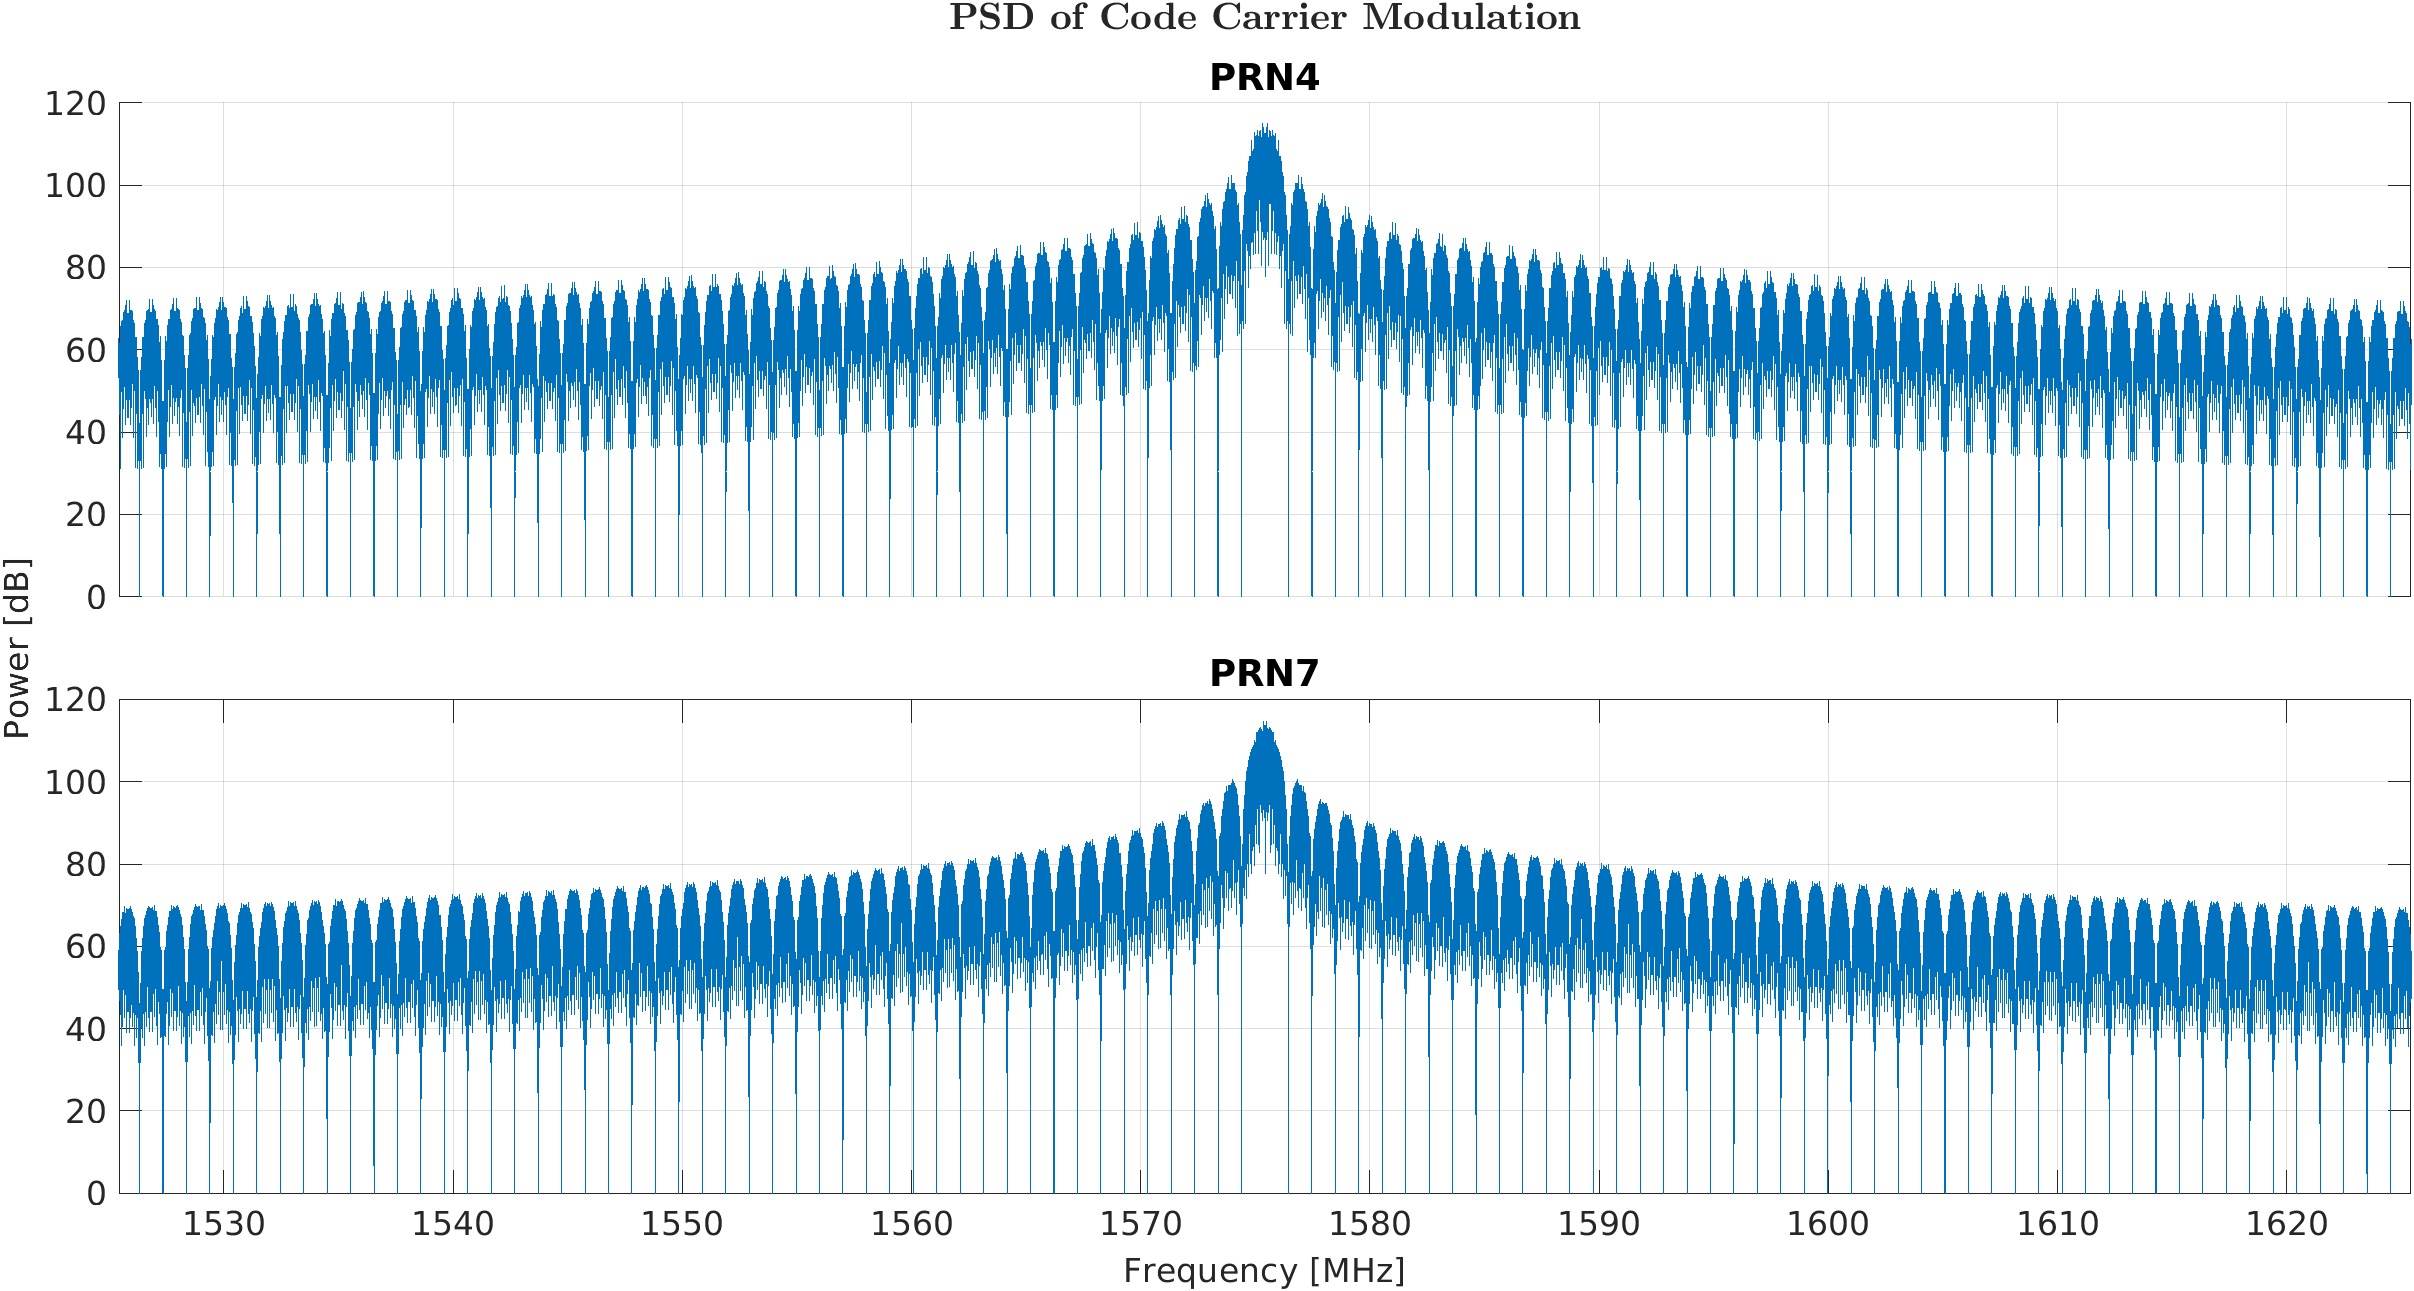
\includegraphics[width=0.85\textwidth]{8.png}
    \caption{Code - Carrier Modulation}
  \end{figure}
  
\end{enumerate}

\end{document}